\documentclass[lettersize,journal]{IEEEtran}
\usepackage{amsmath,amsfonts}
\usepackage{stix}
\usepackage{algorithmic}
\usepackage{algorithm}
\usepackage{array}
\usepackage[caption=false,font=normalsize,labelfont=rm,textfont=sf]{subfig}
\usepackage{textcomp}
\usepackage{stfloats}
\usepackage{url}
\usepackage{verbatim}
\usepackage{graphicx}
\usepackage{cite}

\usepackage{multirow}
\usepackage{booktabs}
\usepackage{makecell}

\usepackage[backref]{hyperref} 
\hyphenation{op-tical net-works semi-conduc-tor IEEE-Xplore}
% updated with editorial comments 8/9/2021

\begin{document}

\title{Zig-zag Scanline Level Parallelized RDOQ Algorithm and its Pipelined Hardware Architecture Design for AVS3 Video Coding}

\author{Xiaofeng Huang, Ran Tang, Rui Pan, Haibing Yin, Zhao Wang, Shiqi Wang, Siwei Ma
% \author{IEEE Publication Technology,~\IEEEmembership{Staff,~IEEE,}
        % <-this % stops a space
\thanks{This work was supported in part by the National Natural Science Foundation of China under Grant 61901150, 61931008, and 61972123, and in part by the National Key R\&D Program of China under Grant 2021ZD0109802.}% <-this % stops a space
\thanks{Xiaofeng Huang, Ran Tang, Haibing Yin, and Chenggang Yan are
with the School of Communication Engineering, Hangzhou Dianzi University,
Hangzhou 310018, China (e-mail: \{xfhuang; wh\_niu; 192080054; yhb\}@hdu.edu.cn).}
\thanks{Guoqing Xiang is with the Advanced Institute of Information Technology, Peking University,
Hangzhou 311215, China (e-mail: gqxiang@pku.edu.cn).}
\thanks{Siwei Ma is with the School of Computer Science, Peking University,
Beijing 100871, China (e-mail: swma@pku.edu.cn).}
%\thanks{This paper was produced by the IEEE Publication Technology Group. They are in Piscataway, NJ.}% <-this % stops a space
%\thanks{Manuscript received April 19, 2021; revised August 16, 2021.}
}

% The paper headers
\markboth{Journal of \LaTeX\ Class Files,~Vol.~14, No.~8, August~2021}%
{Shell \MakeLowercase{\textit{et al.}}: A Sample Article Using IEEEtran.cls for IEEE Journals}

\IEEEpubid{0000--0000/00\$00.00~\copyright~2021 IEEE}
% Remember, if you use this you must call \IEEEpubidadjcol in the second
% column for its text to clear the IEEEpubid mark.

\maketitle

\begin{abstract}

The rate-distortion optimized quantization (RDOQ) provides significant coding gain in the third generation of Audio Video coding Standard (AVS3). However, the high computational complexity and strong data dependency in RDOQ impede the hardware implementation. To address these issues, we propose a zig-zag scanline-level parallelized RDOQ algorithm and its fully pipelined hardware architecture for AVS3 video coding. For algorithm optimization, we update the run-level context for rate estimation in the inner zig-zag scanline and adopt an efficient RD cost form in the optimal coefficient level (OCL) decision. In the last significant coefficient (LSC) position decision, a greedy strategy-based algorithm is proposed to calculate the determination in parallel. Moreover, the proposed parallelized RDOQ algorithm is accelerated by single incrustation multiple data (SIMD) on the Intel X86 platform. \emph{TODO: hardwareMoreover, the hardware architecture is implemented in Verilog based on the proposed parallelized algorithm. It can support the real-time encoding requirements for 4K@30fps. It is evident that a good trade-off exists between coding efficiency and hardware throughput.} Experimental results show that the proposed algorithm achieves 31.42\%, 28.60\%, and 28.58\% time-saving by a 0.23\%, 0.24\%, and 0.26\% Bjøntegaard delta rate (BD-rate) increase on average under All-Intra (AI), Random-Access (RA), and Low-Delay B (LDB) configurations, respectively. 


% which also suffers from a high computational complexity and strong data dependency hinders hardware implementation. To address the issues, we propose a zig-zag scanline level parallelied RDOQ algorithm and its pipelined hardware architecture. For algorithm optimization, the run-level context for the rate estimation is updated in the inner zig-zag scanline and an efficient RD cost form is adopted in the optimal coefficient level (OCL) decision step. In the last significant coefficient (LSC) position decision step, a greedy strategy-based algorithm is proposed to enable the LSC position to be calculated in parallel. Meanwhile, the improved RDOQ process is accelerated based on SIMD. The experimental results show that compared with HPM-4.0.1, the proposed algorithm can achieves a 0.23\%, 0.24\% and 0.26\% Bjøntegaard delta rate (BD-rate) loss and a 31.42\%, 28.60\% and 28.58\% average RDOQ time-saving under All-Intra (AI), Random-Access (RA) and Low-Delay B (LDB) configurations, respectively.
% Moreover, the hardware architecture is implemented in Verilog base on the proposed parallelized algorithm. It can support the real-time encoding requirements for 4K@30fps. It is evident that a good trade-off exists between coding efficiency and hardware throughput.
\end{abstract}

\begin{IEEEkeywords}
	RDOQ, AVS3, zig-zag scanline, parallelized algorithm, hardware architecture.
\end{IEEEkeywords}

\section{Introduction}
\label{sec:1}
\IEEEPARstart{W}{ith} the growing popularity of ultra-high definition (UHD) video content such as 4K and 8K, the amount of video data has shown an explosive increment. According to Cisco's report, video data accounted for 82\% of all mobile data traffic in 2022, up from 59\% in 2017 \cite{barnett2018cisco}. This has resulted in an urgent need for more advanced video compression coding tools that can provide high compression efficiency to alleviate the burden of video data transmission and storage. To address this challenge, several standard groups have established novel video coding standards. The Joint Video Exploration Team (JVET) formed by the ISO/IEC Moving Picture Experts Group (MPEG) and ITU-T Video Coding Experts Group (VCEG) has developed several video coding standards \cite{1994H.262/MPEG-2, avcoverview, sullivan2012hevcoverview}, and the latest one is called Versatile Video Coding (VVC) \cite{bross2021vvcoverview}. The Chinese AVS working group officially initiated the next-generation video coding standard - AVS3 in March 2018 and finalized the first phase of AVS3 in 2019 \cite{zhang2019avs3overview}. These video coding standards enable more efficient transmission and storage of video data while maintaining high video quality. 

The AVS3 standard is an improvement over its predecessor AVS2, which aims to provide better video compression capability and support for broader video services like virtual reality (VR). To achieve better coding efficiency, several advanced coding tools have been adopted in AVS3. In block partitioning, AVS3 extends the quadtree partition in AVS2 to a more flexible partition mechanism, including quadtree (QT), binary tree (BT) \cite{huang2019vvcbt}, and extended quadtree (EQT) partition \cite{wang2019extendedpartition}. The QT/BT combined with the EQT partition allows the appearance of a non-square coding unit (CU), which makes the CU partition adapt to the video content better. In intra-coding, new coding tools including intra-derived tree (Intra-DT), intra-prediction filter (IPF), and two-step cross-component prediction mode (TSCPM) are specially designed for AVS3. In inter coding, AVS3 introduces adaptive motion vector resolution (AMVR), enhanced motion vector resolution (EMVR), and affine motion mode, which improve the efficiency of temporal redundancy removal \cite{fan2020avs3codingtools}. In transform coding, more transform types like DST-VII and DCT-VIII are supported in AVS3 \cite{avs3standard}. These advanced coding tools make AVS3 show a significant improvement over AVS2 in terms of compression efficiency. 

\IEEEpubidadjcol

In addition to the advanced coding tools mentioned above, AVS3 adopts rate-distortion optimized quantization (RDOQ) to further improve coding efficiency. RDOQ offers significant performance gains compared to conventional uniform scalar quantization (USQ). The coding gain is achieved by searching for the best coefficient level and last significant coefficient position in a rate-distortion (RD) optimal way. Specifically, to determine the optimal quantization level for each transform coefficient, RDOQ repeatedly computes the RD cost for all possible candidate levels. The rate cost is computed sequentially due to entropy coding with context model update. Similarly, the decision-making process for the last significant coefficient position is also sequential as all the quantized coefficients are searched one by one. The position with the minimum summed RD cost is chosen as the optimal one. The coefficients are accessed in zig-zag scan order during the RDOQ process, which yields memory access conflicts when trying to parallelize in hardware implementation. As a result, the high computational complexity of RDOQ and its sequential processing characteristics pose challenges for real-time video coding applications. 

Over the past decade, numerous researchers have attempted to simplify the RDOQ process in different ways to reduce its computational complexity \cite{yin2014fasttrellis, wang2017fast, yin2019efficient, wang2021trellis}. These optimization methods can be classified into two main categories, bypass RDOQ and fast RDOQ. Bypass RDOQ skips the RDOQ process entirely by utilizing techniques such as zero block detection. In contrast, fast RDOQ seeks to simplify the computation process within RDOQ. From another perspective, existing methods can be classified as software or hardware-based, depending on the target optimization platform. The research on RDOQ is summarized in Fig.~\ref{summary}. 

In the bypass RDOQ methods, pieces of research skip the redundant process by pre-detecting all-zero blocks to reduce the computational complexity \cite{lee2016all-zero, wang2017fastrdoq}. In \cite{fan2016hybridzreoblock, cui2018hybrid}, these two works detect genuine all-zero block (GZB) and pseudo all-zero block (PZB) to early terminate the process. Work \cite{fan2016hybridzreoblock} introduced a sum of absolute difference (SAD) lower bound as a threshold to detect GZB and proposed an RD estimation method to detect PZB. However, several empirical values were introduced in \cite{fan2016hybridzreoblock} which tends to be sensitive to the initial values. To resolve this problem, work \cite{cui2018hybrid} proposed a PZB detection method, where rate-distortion optimization (RDO) with adaptive RD estimation is employed. Similarly, works \cite{cui2017adaptive, wei2019all} utilized the maximum transform coefficient in the transform block as the threshold for fast AZB detection. To improve the detection accuracy, multi-stage all-zero block detection methods are proposed in \cite{yin2018efficient, yin2020multistageallzerodetection}. Work \cite{yin2018efficient} proposed a coefficient-level zero-quantized threshold model by fully simulating RDOQ for AZB detection. And, multi-stage AZB detection using a machine learning model was introduced in \cite{yin2020multistageallzerodetection}, where a model was offline trained for all-zero block determination based on eight influenced features. For the blocks with few RDOQ coding gains, works \cite{lee2015fastquantizationmethod, zhang2015fastrdoq} used USQ instead of RDOQ directly. For the coefficient-level RDOQ bypass method, works \cite{xu2018simplifiedrdoq, xu2020simplifiedLevelEstimation} proposed an adaptive dead zone offset to adjust the quantization level from one to zero at the high-frequency domain in large transform blocks. These algorithms can save significant computational time on certain conditions, but the processing logic is still redundant when the condition is not met. Therefore, these bypass RDOQ methods are of limited use for real-time hardware RDOQ applications, as the sequential and redundant processing is still the bottleneck when implemented in hardware. 

In the fast RDOQ methods, they focus on the simplification of RD calculation. Rate estimation in RDOQ is usually derived by the entropy coding with context model update which impedes parallel computing. To resolve this problem, work \cite{huang2015efficientquantization} proposed a rate model through an analytical method to speed up the RDOQ, and it can predict the bitrate by different entropy coding methods. However, the method \cite{huang2015efficientquantization} is no longer suitable for HEVC as HEVC has more complex transform types. Therefore, work \cite{cui2017Laplacedistributionbased} proposed a low-complexity RDOQ optimization algorithm based on a hybrid Laplacian model. An alternative approach is to calculate the difference of RD cost between two candidate quantized levels, rather than calculating the two RD costs separately \cite{he2015highimplementationrdoq}. Similarly, works \cite{lee2015fastquantizationmethod} and \cite{wang2016improvedrdoq} built a low-complexity $\Delta$J model based on syntax elements involved in the rate estimation, which significantly reduce encoder complexity during the RDOQ process. Moreover, works \cite{canh2018rate} and \cite{kianfar2020parallelized} accelerate the RDOQ process utilizing deep learning methods. In work \cite{canh2018rate}, the optimal quantization level was determined using a residual depth convolutional neural network, eliminating the need for RD cost calculation. Work \cite{kianfar2020parallelized} trained neural networks to predict an additive adjustment value per transform coefficient, and the networks had fewer parameters compared to \cite{canh2018rate}. 

From Fig.~\ref{summary}, it is evident that most of the current fast algorithms are developed for software platforms, while only a few are designed for hardware platforms. Work \cite{igarashi2018parallelGPU} parallelized the RD cost calculation by utilizing the entropy at the previous frame and utilized a bi-directional (forward and reverse) parallel scan to accumulate the RD cost for the last significant coefficient position search. It can achieve 4K@60fps real-time processing on GPU, but it comes with a significant 2.6\% increase in Bjøntegaard delta Rate (BD-rate) \cite{bjontegaard2001calculationofPSNR}. In \cite{xu2022hardwarefriendlyforrdoq}, a hardware-friendly fast RDOQ algorithm for AVS3 is proposed. It eliminates the data dependency during rate estimation, but the optimization of the last significant coefficient position search has not been addressed which poses challenges for parallel implementation in hardware. In our previous work \cite{zhao2023scanline}, we proposed a zig-zag scanline-based fast algorithm and its hardware implementation. However, to facilitate hardware implementation, we fixed the context during RDOQ processing, which resulted in a 0.5\% BD-rate increase. 

%\par
\begin{figure}[!h]
	\centering
	\centerline{\includegraphics[width=0.48\textwidth]{figure/Summary_rdoq.png}} 
	\caption{Summary of the existing research on RDOQ.}
	\label{summary} % Give a unique label
\end{figure}
\par
In this work, we propose a zig-zag scanline level parallelized RDOQ algorithm and its fully pipelined hardware architecture design for the AVS3 video encoder. Our parallelized algorithm achieves significant time savings with only a slight BD-Rate loss. Compared with the vanilla HPM-4.0.1 software, our algorithm increases BD-Rate by 0.23\%, 0.24\%, and 0.26\% and saves RDOQ time by 31.42\%, 28.60\%, and 28.58\% under All-Intra (AI), Random-Access (RA), and Low-Delay B (LDB) configurations, respectively. Unlike existing bypass and fast RDOQ algorithm \cite{lee2016all-zero, wang2017fastrdoq, fan2016hybridzreoblock, cui2018hybrid, cui2017adaptive, wei2019all, yin2018efficient, yin2020multistageallzerodetection, lee2015fastquantizationmethod, zhang2015fastrdoq, xu2018simplifiedrdoq, xu2020simplifiedLevelEstimation, huang2015efficientquantization, cui2017Laplacedistributionbased, he2015highimplementationrdoq, wang2016improvedrdoq, canh2018rate, kianfar2020parallelized}, our algorithm is more friendly for the efficient hardware implementation. \emph{TODO: hardware related description. } The algorithm improves the accuracy compared with the hardware-oriented implementation in \cite{igarashi2018parallelGPU, xu2022hardwarefriendlyforrdoq}, and \cite{zhao2023scanline}. The main contributions of this work are summarized as follows. 

% In this work, an FPGA-based 4K@30fps real-time high-parallelism RDOQ algorithm and the corresponding hardware architecture are proposed for the AVS3 encoder. First, from an algorithm point of view, Our proposed parallelized algorithm significantly achieved time saving at a slight BD-Rate loss. Compared with the HPM-4.0.1 software, the proposed parallelized algorithm leads to a 0.23\%, 0.24\% and 0.26\% BD-Rate loss and a 31.42\%, 28.60\% and 28.58\% average RDOQ time-saving under All-Intra (AI), Random-Access (RA) and Low-Delay B (LDB) configurations, respectively. Moreover, unlike these bypass and fast algorithm \cite{lee2016all-zero, wang2017fastrdoq, fan2016hybridzreoblock, cui2018hybrid, cui2017adaptive, wei2019all, yin2018efficient, yin2020multistageallzerodetection, lee2015fastquantizationmethod, zhang2015fastrdoq, xu2018simplifiedrdoq, xu2020simplifiedLevelEstimation, huang2015efficientquantization, cui2017Laplacedistributionbased, he2015highimplementationrdoq, wang2016improvedrdoq, canh2018rate, kianfar2020parallelized}, our proposed algorithm is friendly to apply to an efficient hardware architecture. Second, from a hardware architecture perspective, \emph{TODO: hardware architecture}

\begin{enumerate}[]
	\item In the OCL decision step, the run-level context dependency for the rate estimation is optimized to the inner zig-zag scanline level and an efficient RD cost form is adopted to optimize bit-width and rate cost calculation. It simplifies the computational complexity of OCL decision and parallelized the calcuation at scanline level.
 % updated in the inner zig-zag scanline and an efficient RD cost form is adopted, which simplify the computational complexity of OCL decision for parallel purpose.
	\item In the LSC position decision step, a greedy strategy-based algorithm is proposed. It searches the optimal LSC position $i_{k}^{*}$ at a scanline $k$, and the determines the optimal LSC postion $i$ from these $i_{k}^{*}$ candidates. It enables the parallelized computation of LSC position decision. Moreover, the proposed algorithm is further accelerated by single instruction multiple data (SIMD) on Intel X86 platform, which obtains significant time-saving. 
	% \item The proposed algorithm is hardware friendly and also considers the RD performance, the detailed test results are given in Section \ref{sec:5}. Moreover, the algorithm improves the accuracy compared with the hardware-oriented implementation in \cite{igarashi2018parallelGPU, xu2022hardwarefriendlyforrdoq}, and \cite{zhao2023scanline}.
	\item The proposed hardware architecture is described in Verilog and synthesized in FPGA. It configurable to the all TU sizes is designed, which also fills the gap with a good trade-off between hardware implementation and coding performance, and provides a reference for RDOQ-related algorithms, such as soft decision quantization (SDQ) or dependent quantization (DQ), to be implemented on hardware in the future.
\end{enumerate}
\par
The rest of this paper is organized as follows. The RDOQ process in AVS3 and its hardware design challenges are briefly described in Section \ref{sec:2}. Section \ref{sec:3} analyzes the proposed parallelized RDOQ algorithm, and Section \ref{sec:4} gives the hardware architecture design and timing diagrams. The experiment results and comparisons under the common conditions are showed in Section \ref{sec:5}, followed by the conclusion and future work in Section \ref{sec:6}. 

\section{Rate-Distortion Optimized Quantization \\ in AVS3}
\label{sec:2}
In this section, we will first provide an overview of the AVS3 RDOQ process, followed by an analysis of the challenges that arise during hardware design. 
\subsection{AVS3 RDOQ Overview}
\label{sec:2A}
RDOQ is a soft quantization decision technique that aims to find out the optimal quantized coefficient level considering a tradeoff between rate and distortion  \cite{zhao2023scanline},\cite{huang2023rate}. The flow of the RDOQ in AVS3 is shown in Fig.~\ref{rdoq process}. This flow is similar to RDOQ in HEVC \cite{cui2017Laplacedistributionbased} but differs in two crucial ways. One is that the transform unit (TU) level zig-zag scan order is adopted by AVS3, instead of the coefficient group (CG) scan in HEVC. An example is shown in Fig.~\ref{scan}. The other is that AVS3 supports rectangular blocks such as $16\times8$ and $64\times8$. The detailed AVS3 RDOQ flow in Fig.~\ref{rdoq process} consists of four internal components, which are pre-quantization, optimal coefficient level (OCL) decision, last significant coefficient (LSC) position decision, and uncoded coefficient zero assignment. 
\par
\begin{figure}[!h]
	\centering
	\centerline{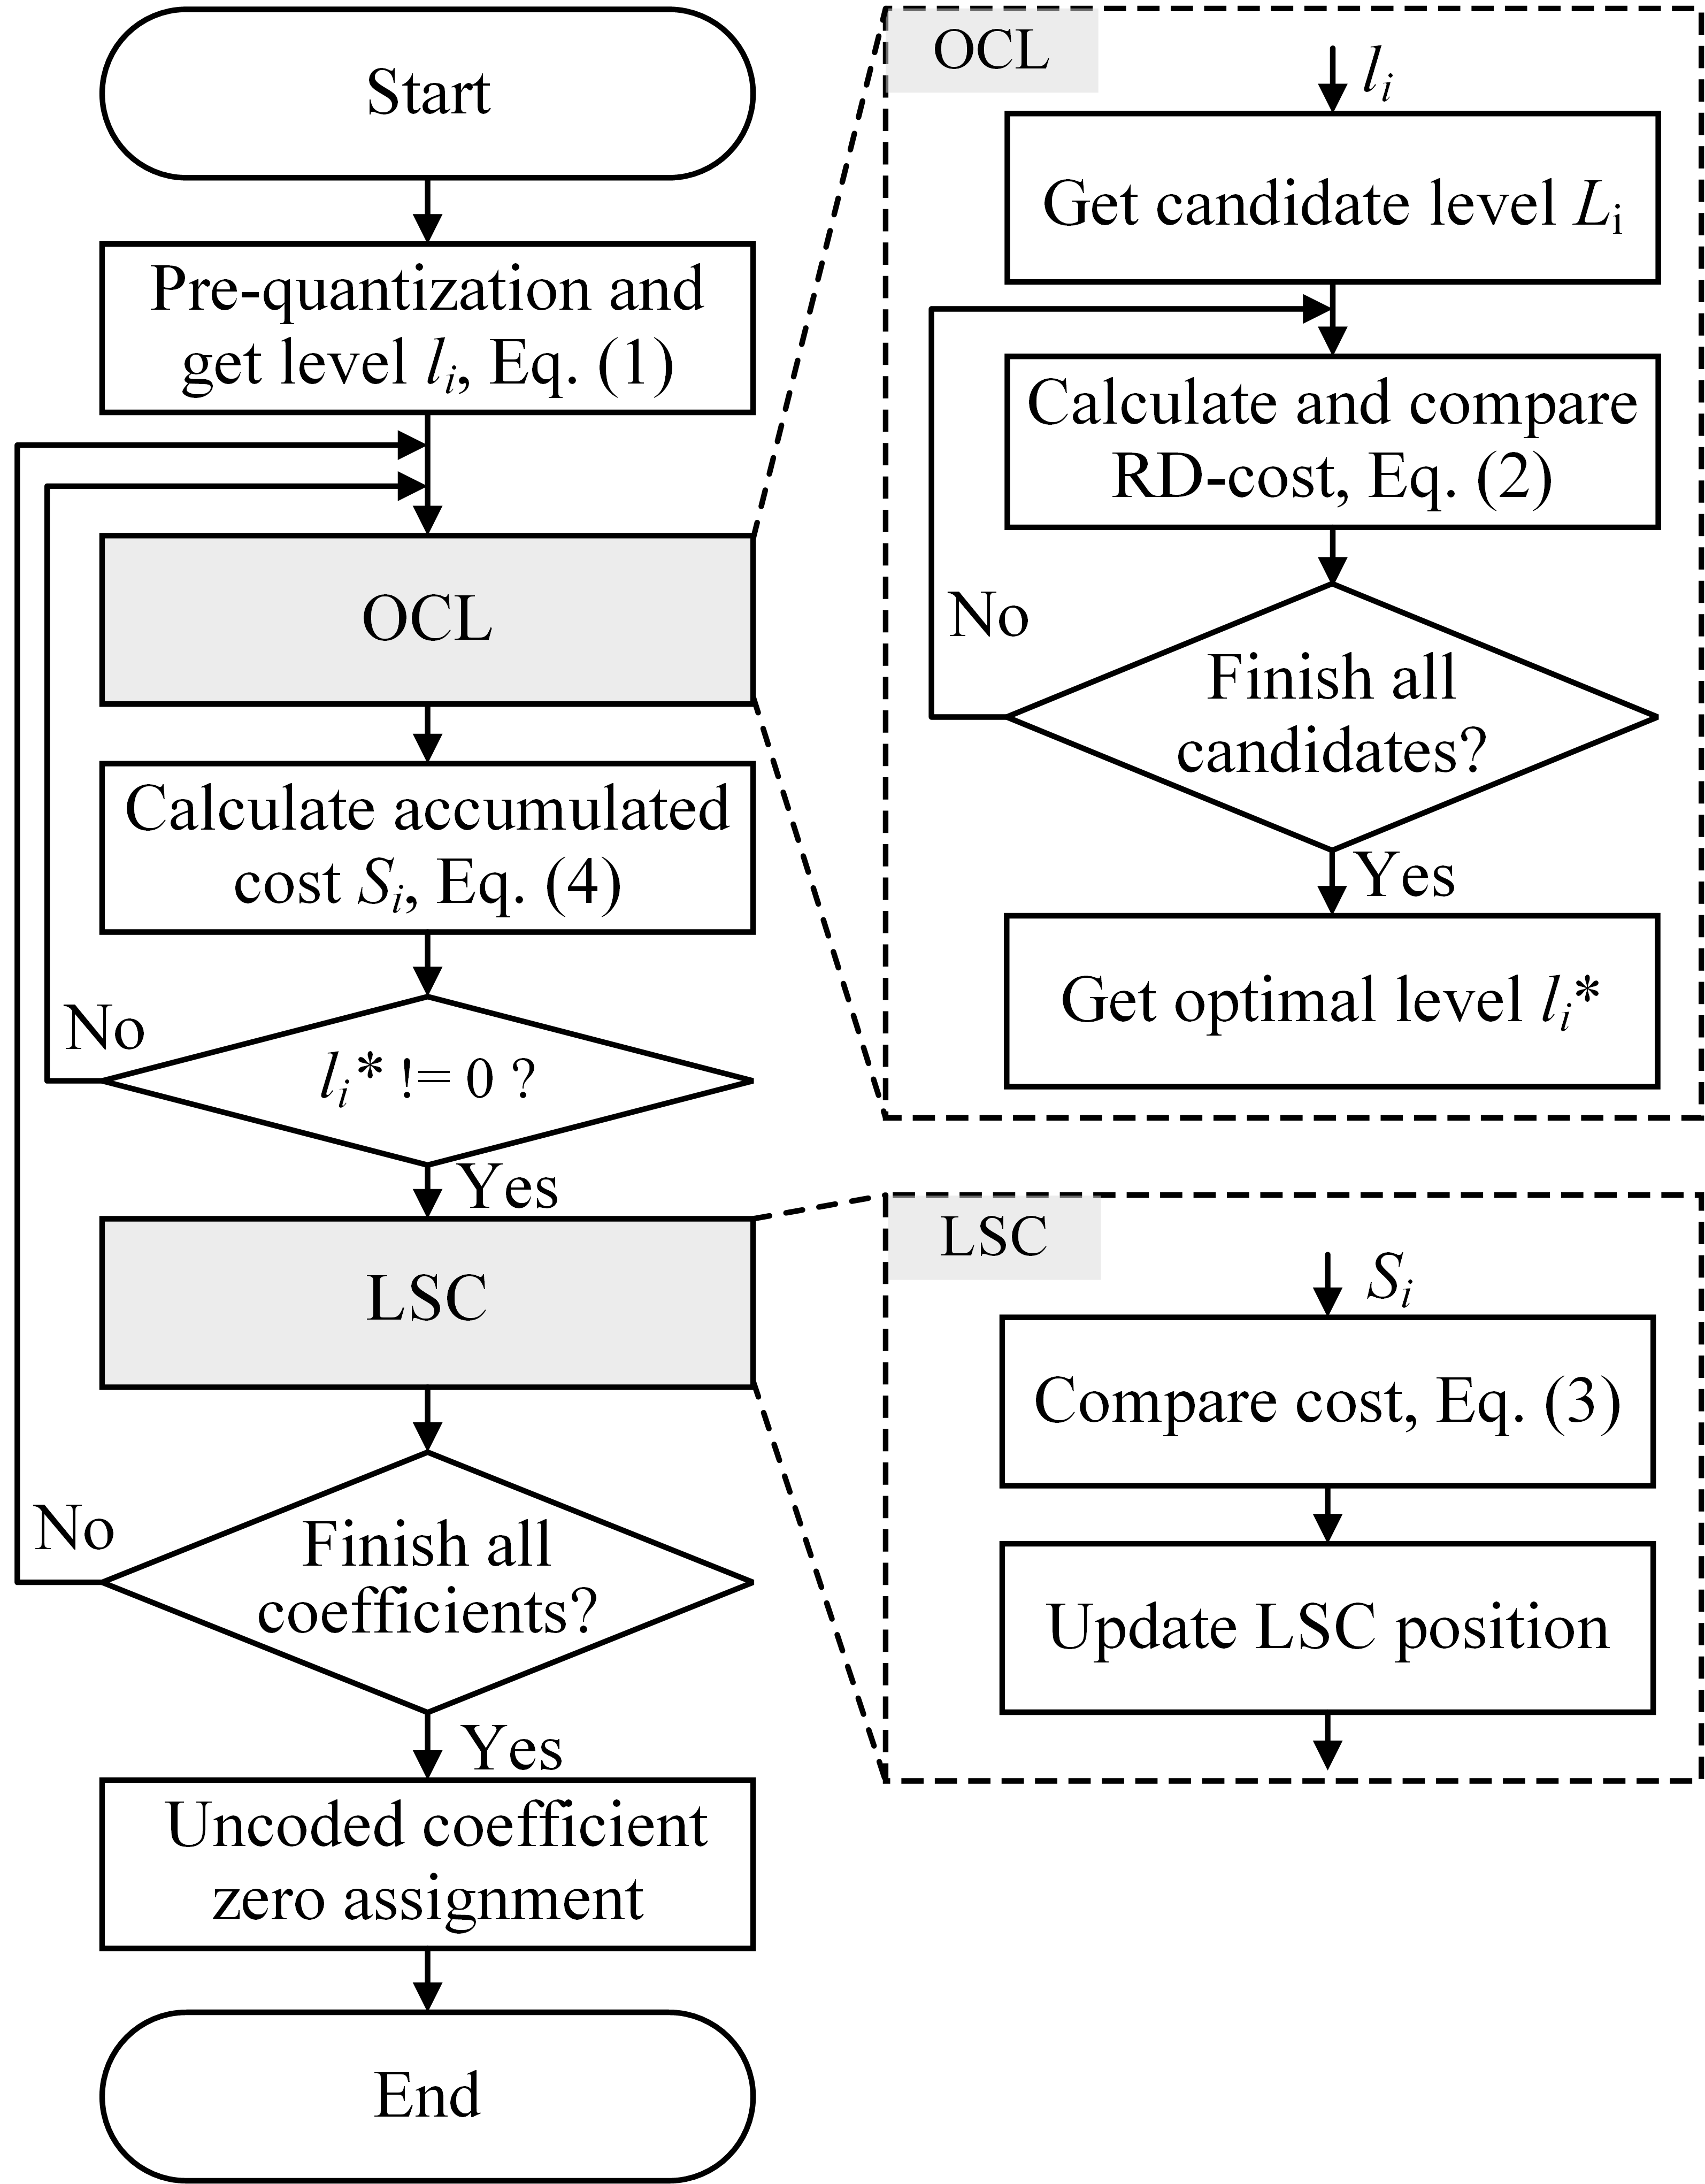
\includegraphics[width=0.42\textwidth]{figure/OriRDOQ.png}} 
	% figure caption is below the figure
	\caption{Flowchart of the RDOQ in AVS3.}
	\label{rdoq process} % Give a unique label
\end{figure}
In the pre-quantization step, each transform coefficient $c_{i}$ located at the zig-zag scan index $i$ in the TU undergoes a scalar quantization which is formulated as, 
\begin{equation}
\label{round}
l _{i} = Round\left ( \frac{\left | c_{i}  \right | }{Q_{step} } +  f \right ),
\end{equation}
where $Q_{step}$ is the quantization step size determined by the quantization parameter (QP), $f$ is the rounding offset, and $l _{i}$ is the initial scalar quantization level. 

In the OCL decision step, the optimal quantization level $l_{i}^{*}$ is determined by comparing the RD cost of available candidate levels $L_{i}$. The derivation of $L_{i}$ is listed in Table~\ref{tab:candidate list}. The level with the minimum cost is selected as the optimal choice. The OCL process is detailed as follows, 
\begin{equation}
\label{rdcost}
l_{i}^{*}  =\mathop{\arg\min}\limits_{L_{i} } \ J, \quad where \quad J=D+\lambda \cdot R,
% l_{i}^{*}  =\mathop{\arg\min}\limits_{L_{i} } \left \{ D+\lambda \cdot R   \right \} 
% \min_{l_{i} \in L_{i}  } \left \{ J \right \} , \quad where \quad J=D+\lambda \cdot R
\end{equation}
where $R$ and $D$ are the rate and distortion, $\lambda$ is the Lagrangian multiplier associated with the QP, and $J$ is the calculated RD cost, respectively. Specifically, the rate $R$ is derived through entropy coding with a context model update. In the AVS3 reference software HPM-4.0.1, the rate $R$ is estimated using a look-up-table, where the table index is determined based on the run-level context update \cite{wang2013transform, wang2019coding}. 
\begin{table}[!ht]
	%\usepackage{hhline}
	\caption{derivation of candidate levels\label{tab:candidate list}}
	\centering
	\tabcolsep 10pt  % 
	\arrayrulewidth 0.75pt
	\begin{tabular}{c | c}
		\midrule[0.75pt] \specialrule{0em}{0.35pt}{0.35pt} \midrule[0.75pt] % \toprule
		\textbf{$l _{i} $} & candidate levels ($L _{i}$) \\ \midrule[0.75pt] 
		0      & N/A                    \\ \midrule[0.75pt]
		1      & 0, 1                   \\ \midrule[0.75pt]
		2      & 0, 1, 2                \\ \midrule[0.75pt]
		...    & ...                  \\ \midrule[0.75pt]
		$N$      & 0, $N$-1, $N$              \\ \midrule[0.75pt] \specialrule{0em}{0.35pt}{0.35pt} \midrule[0.75pt] % \bottomrule
	\end{tabular}
\end{table}

Then in the LSC position decision step, the optimal LSC position $i_{}^{*}$ is derived based on the sum of RD cost. The algorithm scans through each coefficient position $i$ in zig-zag order and determines the optimal position by the following formula,
\begin{figure}[!h]
	\centering
	\centerline{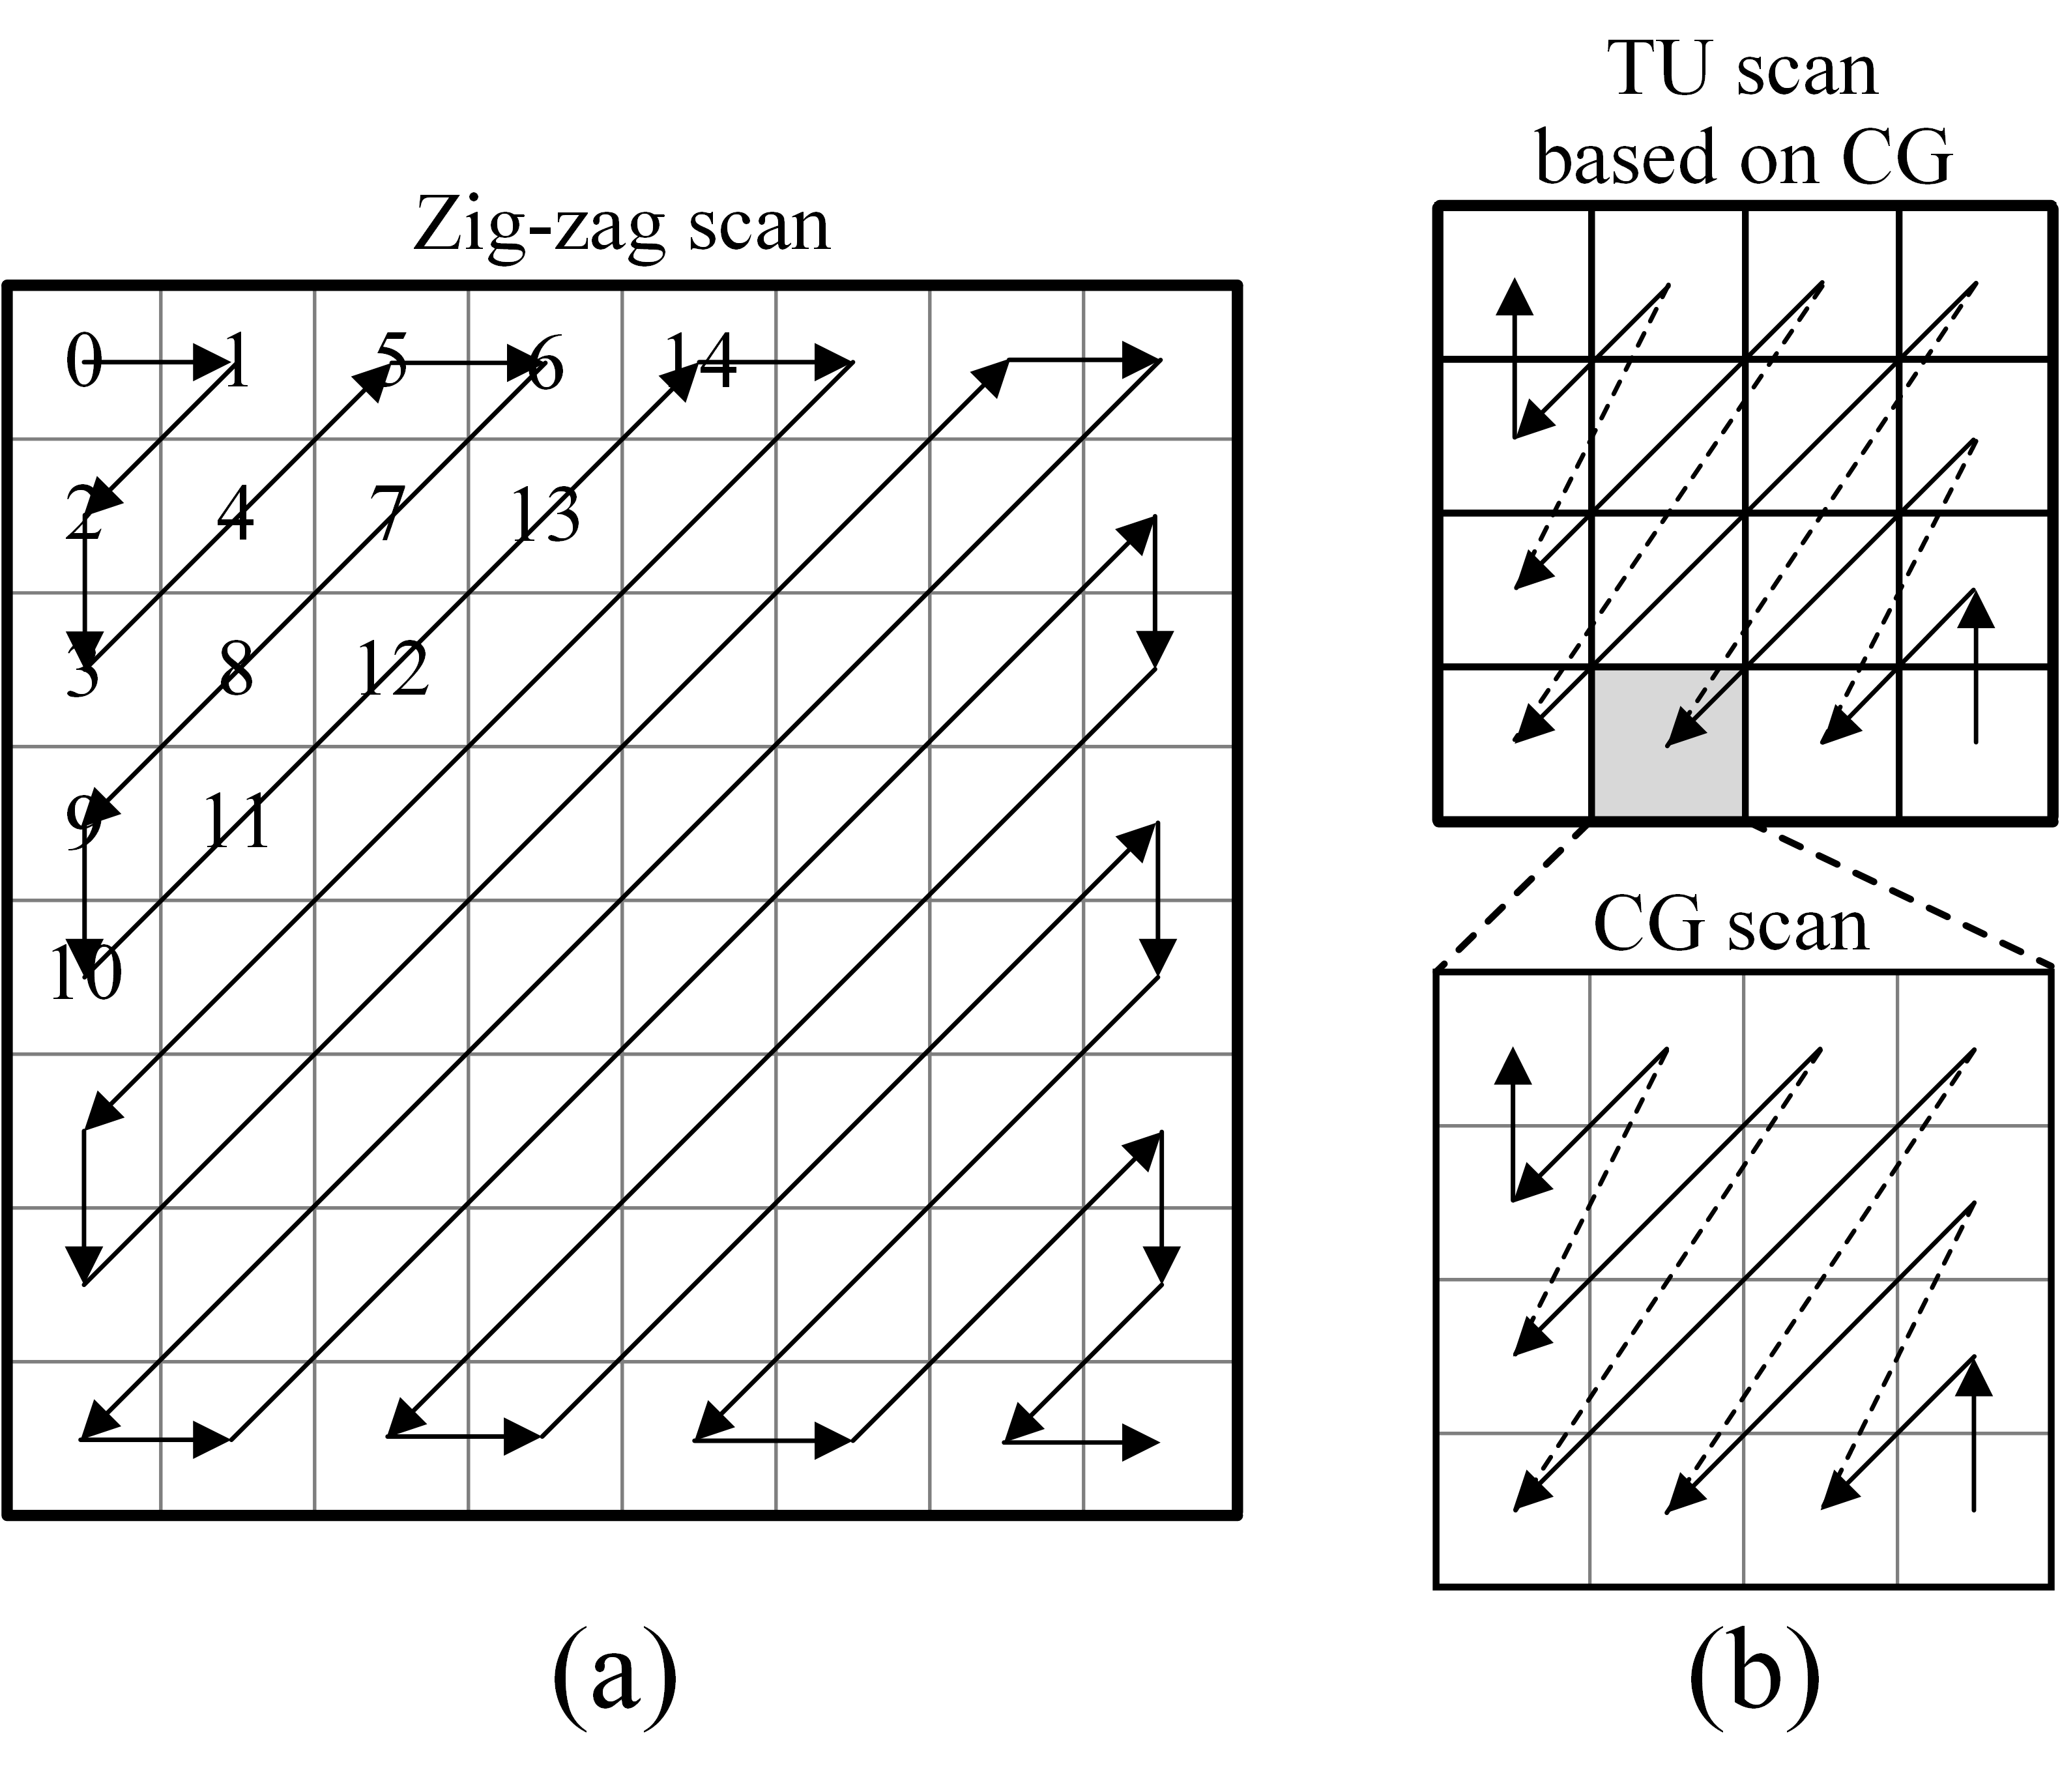
\includegraphics[width=0.45\textwidth]{figure/scan.png}} 
	% figure caption is below the figure
	\caption{Scan order comparison. (a) zig-zag scan in AVS3, (b) CG-based diagonal scan in HEVC.}
	\label{scan} % Give a unique label
\end{figure}

%\begin{equation}
%\begin{aligned}
%\label{optimal}
%&i_{optimal} = \\ &\mathop{\arg\min}\limits_{i\epsilon \left ( firstpos,...,lastpos \right ) } \left \{ \sum_{j=0}^{i}\left ( J_{i,coded} - J_{i,uncoded}\right ) + E_{i,last}   \right \} 
%\end{aligned}
%\end{equation}
\begin{equation}
	\begin{aligned}
		\label{i_optimal}
		i_{}^{*} =\mathop{\arg\min}\limits_{i \in \left \{ 0,...,W\times H-1\right \} } \left ( S_{i} + E_{i,lsc}   \right ),
% i_{optimal} =\mathop{\arg\min}\limits_{i \in \left ( firstpos,...,lastpos \right ) } \left \{ A_{i,cost} + E_{i,last}   \right \} 
	\end{aligned}
\end{equation}
where $W$ and $H$ represent the width and height of the TU, $E_{i,lsc}$ denotes the rate cost of the synatx elemenet $coeff\_last$ with the assumption that $i$ is the LSC position, and $S_{i}$ denotes the accumulated cost of coefficient positions from zero to $i$, respectively. The $S_{i}$ is formulated as follows, 
\begin{equation}
	\begin{aligned}
		\label{A_i,last}
S_{i} = \sum_{j=0}^{i}\left ( \Delta J_{j} \right), \ where \   \Delta J_{j} = J_{j,l_{j}^{*}} - J_{j,0} + E_{j,non\_lsc}
	\end{aligned}
\end{equation}
where $J_{j,l_{j}^{*}}$ is the RD cost when the coefficient level at position $j$ is quantized to $l_{j}^{*}$, $J_{j,0}$ is the distortion cost when the coefficient level is quantized to zero at position $j$, and $E_{j,non\_lsc}$ is the rate cost of the syntax $coeff\_last$ when the position $j$ is not the LSC position, respectively. The value of $E_{j,non\_lsc}$ is set to zero when $j$ is equal to $i$ or $l_{j}^{*}$ is equal to zero. 

Finally, all non-zero coefficients after the LSC position should be set to zero in the uncoded coefficient zero assignment step. 

\subsection{Hardware Design Challenge Analysis}
\label{subsec:B}
RDOQ determines the optimal quantization level based on an RD optimal perspective, which can achieve higher compression efficiency compared to USQ. The process of the RDOQ in AVS3 is shown in Fig.~\ref{rdoq process}, which consists of four steps. The hardware design challenges for these steps are analyzed in this subsection. 

The pre-quantization and uncoded coefficient zero assignment steps in Fig.~\ref{rdoq process} are well suitable for hardware implementation. This is because they do not involve any data dependency. The pre-quantization step can be implemented in parallel since all coefficients can be quantized independently using Eq. (\ref{round}). Similarly, The uncoded coefficient zero assignment process can also be parallelized, where the coefficient level at location $i$ is set to zero when $i$ is larger than $i_{}^{*}$. Moreover, this step can be merged into the inverse quantization process, which can lead to a reduction in pipeline latency \cite{braatz2018high}. 

In the OCL decision step, the RD calculations using Eq. (\ref{rdcost}) are executed to get the optimal level $l_{i}^{*}$. It can be parallelized as the input context for rate estimation is identical for all candidate levels in $L_{i}$. However, it must be processed serially between coefficient positions $i$ and $i+1$. It is because the run-level context for the next coefficient $i+1$ depends on the optimal level $l_{i}^{*}$. Thus, the next coefficient cannot start until the $l_{i}^{*}$ is decided and the context is updated. Similarly, the LSC position decision step cannot be implemented in parallel as the optimal $i_{}^{*}$ derived from Eq. (\ref{i_optimal}) is searched serially for all coefficient positions in zig-zag order. The serial processing hinders the throughput of RDOQ and thereby reduces its overall efficiency. 

Based on the above analysis, the data dependencies in the OCL decision and LSC position decision steps pose challenges to the parallel hardware implementation of RDOQ. Assuming that the pixel parallelism is 1 coefficient/cycle, processing a $32\times32$ TU will require a total of 1024 clock cycles. This is far from pixel parallelism in the hardware implementation of discrete cosine transform (DCT), where the parallelism can be 32 coefficients/cycle \cite{meher2013efficient,fan2019pipelined,Hao2023Multiple}. This pixel parallelism mismatch will reduce the throughput of the pipelined hardware design of the mode decision in video coding, where RDOQ is an essential stage in the mode decision pipeline \cite{sun2017fast,zhang2018efficient,huang2018three,zhang2018highly}.

Several methods have been proposed to address the data dependency problem in RDOQ \cite{igarashi2018parallelGPU,xu2022hardwarefriendlyforrdoq,zhao2023scanline}. They primarily aim to address the dependency issue caused by context update-based rate estimation, utilizing approaches such as fixed context. This allows the OCL decision process to be implemented in parallel between different coefficient positions, at the expense of some coding performance loss. Despite this, it is still challenging to parallelize the LSC position decision process due to two factors. One is that the zig-zag scan order searching in Eq. (\ref{i_optimal}) hinders the parallelism. The transform coefficients output by the previous stage DCT in mode decision pipeline is column first style, which means the coefficients at positions (0, 2, 3, 9, ...) are output in one cycle \cite{fan2019pipelined}. If we try to parallelize the coefficients at positions from $i$ to $i+3$ in one cycle, the coefficients $c_i$ need to be reshaped from column-first style to zig-zag first style. This reshaping process will consume additional clock cycles and memory resources. The other is that the calculation of the accumulated cost $S_{i}$ impedes the parallelism. If we try to achieve parallelism with 4 coefficients/cycle, $S_{i}$, $S_{i+1}$, $S_{i+2}$, and $S_{i+3}$ need to be derived in one cycle. It is obvious that the computational logic is too heavy, and it will become the critical path resulting in worse timing and lower working frequency. 

In this work, we resolve these problems by proposing a zig-zag scanline level paralleled RDOQ algorithm and implementing a fully pipelined hardware architecture design for AVS3 video coding. \emph{TODO: last refine.}

\section{Proposed parallelized RDOQ Algorithm}
\label{sec:3}
In this section, we will discuss a parallelized RDOQ algorithm to speed up the process. In the OCL decision step, the run-level context for rate estimation is updated in the inner zig-zag scanline, and the RD cost formula presented in Eq. (\ref{rdcost}) is optimized to a more efficient form. In the LSC position decision step, a greedy strategy-based algorithm is proposed, which enables the implementation of Eq. (\ref{i_optimal}) in parallel between zig-zag scanlines. Finally, we summarize the parallelized RDOQ algorithm and accelerate the entire process using a SIMD approach. 

\subsection{Parallelized OCL decision} 
\label{subsecOCL:B}
As described in subsection \ref{subsec:B}, the run-level context update during rate estimation hinders the parallelized implementation of the OCL decision step. Specifically, this dependency arises from the use of variables $prev\_level$ and $run$ in HPM-4.0.1. Here, $prev\_level$ represents the former non-zero optimal quantization level, and $run$ denotes the number of zeros between two non-zero quantization coefficients. For example, if the optimal coefficient levels from positions 0 to 4 are (15, 1, 0, 0, 0), the values of $prev\_level$ and $run$ for position 5 are 1 and 3, respectively. In this subsection, we propose a simplified derivation of these two variables in order to enable the parallelization of the OCL decision step. 

Before illustrating the algorithm, we analyze the zig-zag scan in Fig.~\ref{scan}(a). It is observed that the zig-zag scan follows two different directions, either the down-left scan or the up-right scan. These two different scans have different properties in terms of deriving the variables $prev\_level$ and $run$. For coefficients located on the down-left scanline, the calculation of these two variables depends on the coefficients with a column index greater than the current index. On the other hand, for coefficients located on the up-right scanline, the calculation depends on the coefficients with a column index less than the current one. As illustrated in subsection \ref{subsec:B}, the transform coefficients are output from the DCT in the column-first order, meaning that coefficients with smaller column indices are output first. Therefore, different strategies are required to adapt to the two different scan directions. 

For the value of variable $prev\_level$ at a zig-zag scan index $i$, the simplified derivation is formulated as below, 
\begin{equation}
	prev\_level_{i} =\begin{cases}
		\label{prevlevel}
		1,           & if \ (u==0)\ or\ (v==H^{'}) \\
		l_{i},       & elif \ ((u+v)\&1==1)\ and\ (!!l_{i}) \\
		l_{i-1}^{*}, & elif \ ((u+v)\&1==0)\ and\ (!!l_{i-1}^{*}) \\
            1,        & else 
	\end{cases},
\end{equation}
where the ($u, v$) is the coordinate index of the zig-zag scan position $i$, $H^{'}$ is the TU height $H$ minus one, $l_{i}$ is the pre-quantization level at position $i$, $l_{i-1}^{*}$ is the OCL at previous position $i-1$, and the label ! represents the not operation, respectively. 

Similarly, the derivation of the variable $run$ at index $i$ for the up-right scanline ($(u+v)\&1$==0) is formulated as Eq. (\ref{run}). The derivation for the $run_{i}$ at the down-left scanline ($(u+v)\&1$==1) is analogous to the Eq. (\ref{run}), except that it is calculated based on $l_{i+1}^{*}$ and $run_{i+1}$. 
\begin{equation}
	run_{i}=\begin{cases}
	\label{run}
	0,            & if \ ((!!u)\ or \ (v==H^{'}))\ and \ (!!l_{i}) \\
	1,            & elif \ ((!!u)\ or \ (v==H^{'}))\ and \ (!l_{i})\\
	0,            & elif \  (!!l_{i-1}^{*})\\
	run_{i-1}+1,  & else  \\
\end{cases} .
\end{equation}

Based on the above simplification, it is observed that the derivation of variables $prev\_level_{i}$ and $run_{i}$ exhibits the data dependency within a scanline, and it relies on the coefficients where the column index $u$ is smaller than the current column. This implies that the OCL decision process for coefficients at different rows $v$ in one column can be executed in parallel, and the coefficients at different columns should be processed serially. This method can not only enhance the parallelism and preserve the context update for rate estimation but also ensure that the access aligns with the column-first order from DCT. 

Furthermore, the RD cost calculation in Eq. (\ref{rdcost}) is optimized to a more efficient form, which is expressed below, 
\begin{equation}
    J_{f} =\frac{D}{\lambda } + R,
	\label{pRDcost}
\end{equation}
where the $D$ is the distortion that requires multiplication by the scaling factor $err\_scale$ in HPM-4.0.1. The $err\_scale$ is correlated with the QP and TU size and remains constant for a TU. Therefore, the $err\_scale$ and $\lambda$ can be combined to optimize the division operation in Eq. (\ref{pRDcost}) to a multiplication-shift operation. The adoption of $J_{f}$ brings two benefits. One is that it requires a lower bit-width for the representation of RD cost, which is beneficial for the chip area. In our design, the bit-width for $J_{f}$ is limited to 34. The other is that it eliminates the multiplication operation for the rate cost. Compared to the independent calculation for distortion, there are still some data dependencies in the rate estimation according to Eq. (\ref{prevlevel}) and Eq. (\ref{run}). This form benefits the hardware design of rate calculation. 

\subsection{Greedy strategy-based parallelized LSC position decision}
\label{subsecgreedy}
As shown in Fig.~\ref{rdoq process} and Eq.~\eqref{i_optimal}, the optimal last LSC position $i^{*}$ is determined by searching the minimum accumulated RD cost. The cost is accumulated in the zig-zag scan order, and its hardware design challenges are illustrated in subsection \ref{subsec:B}. To overcome these challenges, a greedy strategy-based LSC position decision algorithm is proposed. In this algorithm, the sub-optimal LSC position $i_{k}^{*}$ at a scanline $k$ is derived first as follows, 
\begin{equation}
	\begin{aligned}
		\label{lk_optimal}
		\bigcup_{k=0}^{n} i_{k}^{*} 
		=\mathop{\arg\min}\limits_{i \in \left \{ b(k),...,e(k)\right \} } \left ( \widetilde{S}_{i}+ E_{i,lsc} \right ) 
	\end{aligned}
\end{equation}
and
\begin{equation}
	\begin{aligned}
		\label{S'i,last}
		\widetilde{S}_{i} = \sum_{j=b(k)}^{i}\left ( \Delta J_{j} \right)
	\end{aligned}
\end{equation}
where $n$ is the total number of scanlines in the TU which is equal to $W+H-1$, $\widetilde{S}_{i}$ is the accumulated cost similar to Eq.~\eqref{A_i,last}, and $b(k)$ and $e(k)$ represent the begin and end position on the $k$-th scanline, respectively. For example, the $b(k)$ and $e(k)$ are 6 and 9 for the 3-rd scanline in Fig.~\ref{zig2col}(a), respectively. 
\par
Then, the optimal $i^{*}$ is derived from the candidate positions $i_{k}^{*}$, and the formula is shown in Eq.~\eqref{li_to_lk}. The decision by Eq.~\eqref{i_optimal} can be converted to Eq.~\eqref{li_to_lk}, where the optimal position decision in the whole TU is divided into comparisons among local scanline optimal positions. And, the optimal last coefficient derived by Eq.~\eqref{i_optimal} is the same as Eq.~\eqref{li_to_lk}. This is because the RD cost $J$ is calculated with inner-scanline dependency and does not have any inter-scanline dependency resulting from the OCL decision optimizations in subsection \ref{subsecOCL:B}. 
\begin{equation}
	\begin{aligned}
		\label{li_to_lk}
		i^{*} &=\mathop{\arg\min}\limits_{i \in \left \{  0,...,W \times H - 1 \right \} } \left ( S_{i} + E_{i,lsc}   \right )
		\\&=\mathop{\arg\min}\limits_{i \in \left \{ \bigcup\limits_{k=0}^{n} i_{k}^{*} \right  \} } \left ( S_{i} + E_{i,lsc}   \right ) .
	\end{aligned}
\end{equation}

Eq.~\eqref{lk_optimal} and Eq.~\eqref{li_to_lk} are the keys to our greedy strategy-based LSC position decision. It indicates that the optimal $i^{*}$ is derived from the sub-optimal LSC position $i_{k}^{*}$. Furthermore, the derivation of $i_{k}^{*}$ can be parallelized across different scanlines, as the $J$, $E_{j,lsc}$, and $E_{j,non\_lsc}$ in Eq.~\eqref{lk_optimal} and Eq.~\eqref{S'i,last} are calculated independently between scanlines. 
  \begin{equation}
      \begin{aligned}
      \label{down_left_ik}
    i_{k}^{*} 
    &=\mathop{\arg\min}\limits_{i \in \left \{ b(k),...,e(k)\right \} } \left ( \widetilde{S}_{i}+ E_{i,lsc} \right ) \\
    &=\mathop{\arg\min}\limits_{i \in \left \{ b(k),...,e(k)\right \} } \left ( \sum_{j=b(k)}^{i} \left ( \Delta J_{j} \right) + E_{i,lsc} \right ) \\
    &=\mathop{\arg\min}\limits_{i \in \left \{ b(k),...,e(k)\right \} } \left ( \sum_{j=b(k)}^{e(k)} \left ( \Delta J_{j} \right )  - \sum_{j=i}^{e(k)} \left ( \Delta J_{j} \right ) + E_{i,lsc} \right ) \\
    &=\mathop{\arg\min}\limits_{i \in \left \{ b(k),...,e(k)\right \} } \left ( \widetilde{S}_{e(k)} - \hat{S}_{i}  + E_{i,lsc} \right ) .
      \end{aligned}
  \end{equation}
\par
There is a problem with the derivation of the $i_{k}^{*}$ for the down-left scanline, as it requires accessing the coefficients $c_{i}$ in right-to-left column order. However, the coefficients are generated in inverse order from the DCT. To resolve this problem, the $i_{k}^{*}$ derivation for the down-left scanline is formulated as Eq.~\eqref{down_left_ik}. In this equation, the $\widetilde{S}_{e(k)}$ is the accumulated cost for the entire scanline, which is a constant value for all coefficients in the scanline. Thus, the $\widetilde{S}_{e(k)}$ can be eliminated for $i_{k}^{*}$ calculation. With this optimization, Eq.~\eqref{down_left_ik} uses cost $J$ for coefficients from left to right order, which aligns with the order of the DCT output. To help understand these variables, an illustration is shown in Fig~\ref{abcompare} for the up-right scanline and down-left scanline, respectively. 
\begin{figure}[!ht]
	\centering
	\centerline{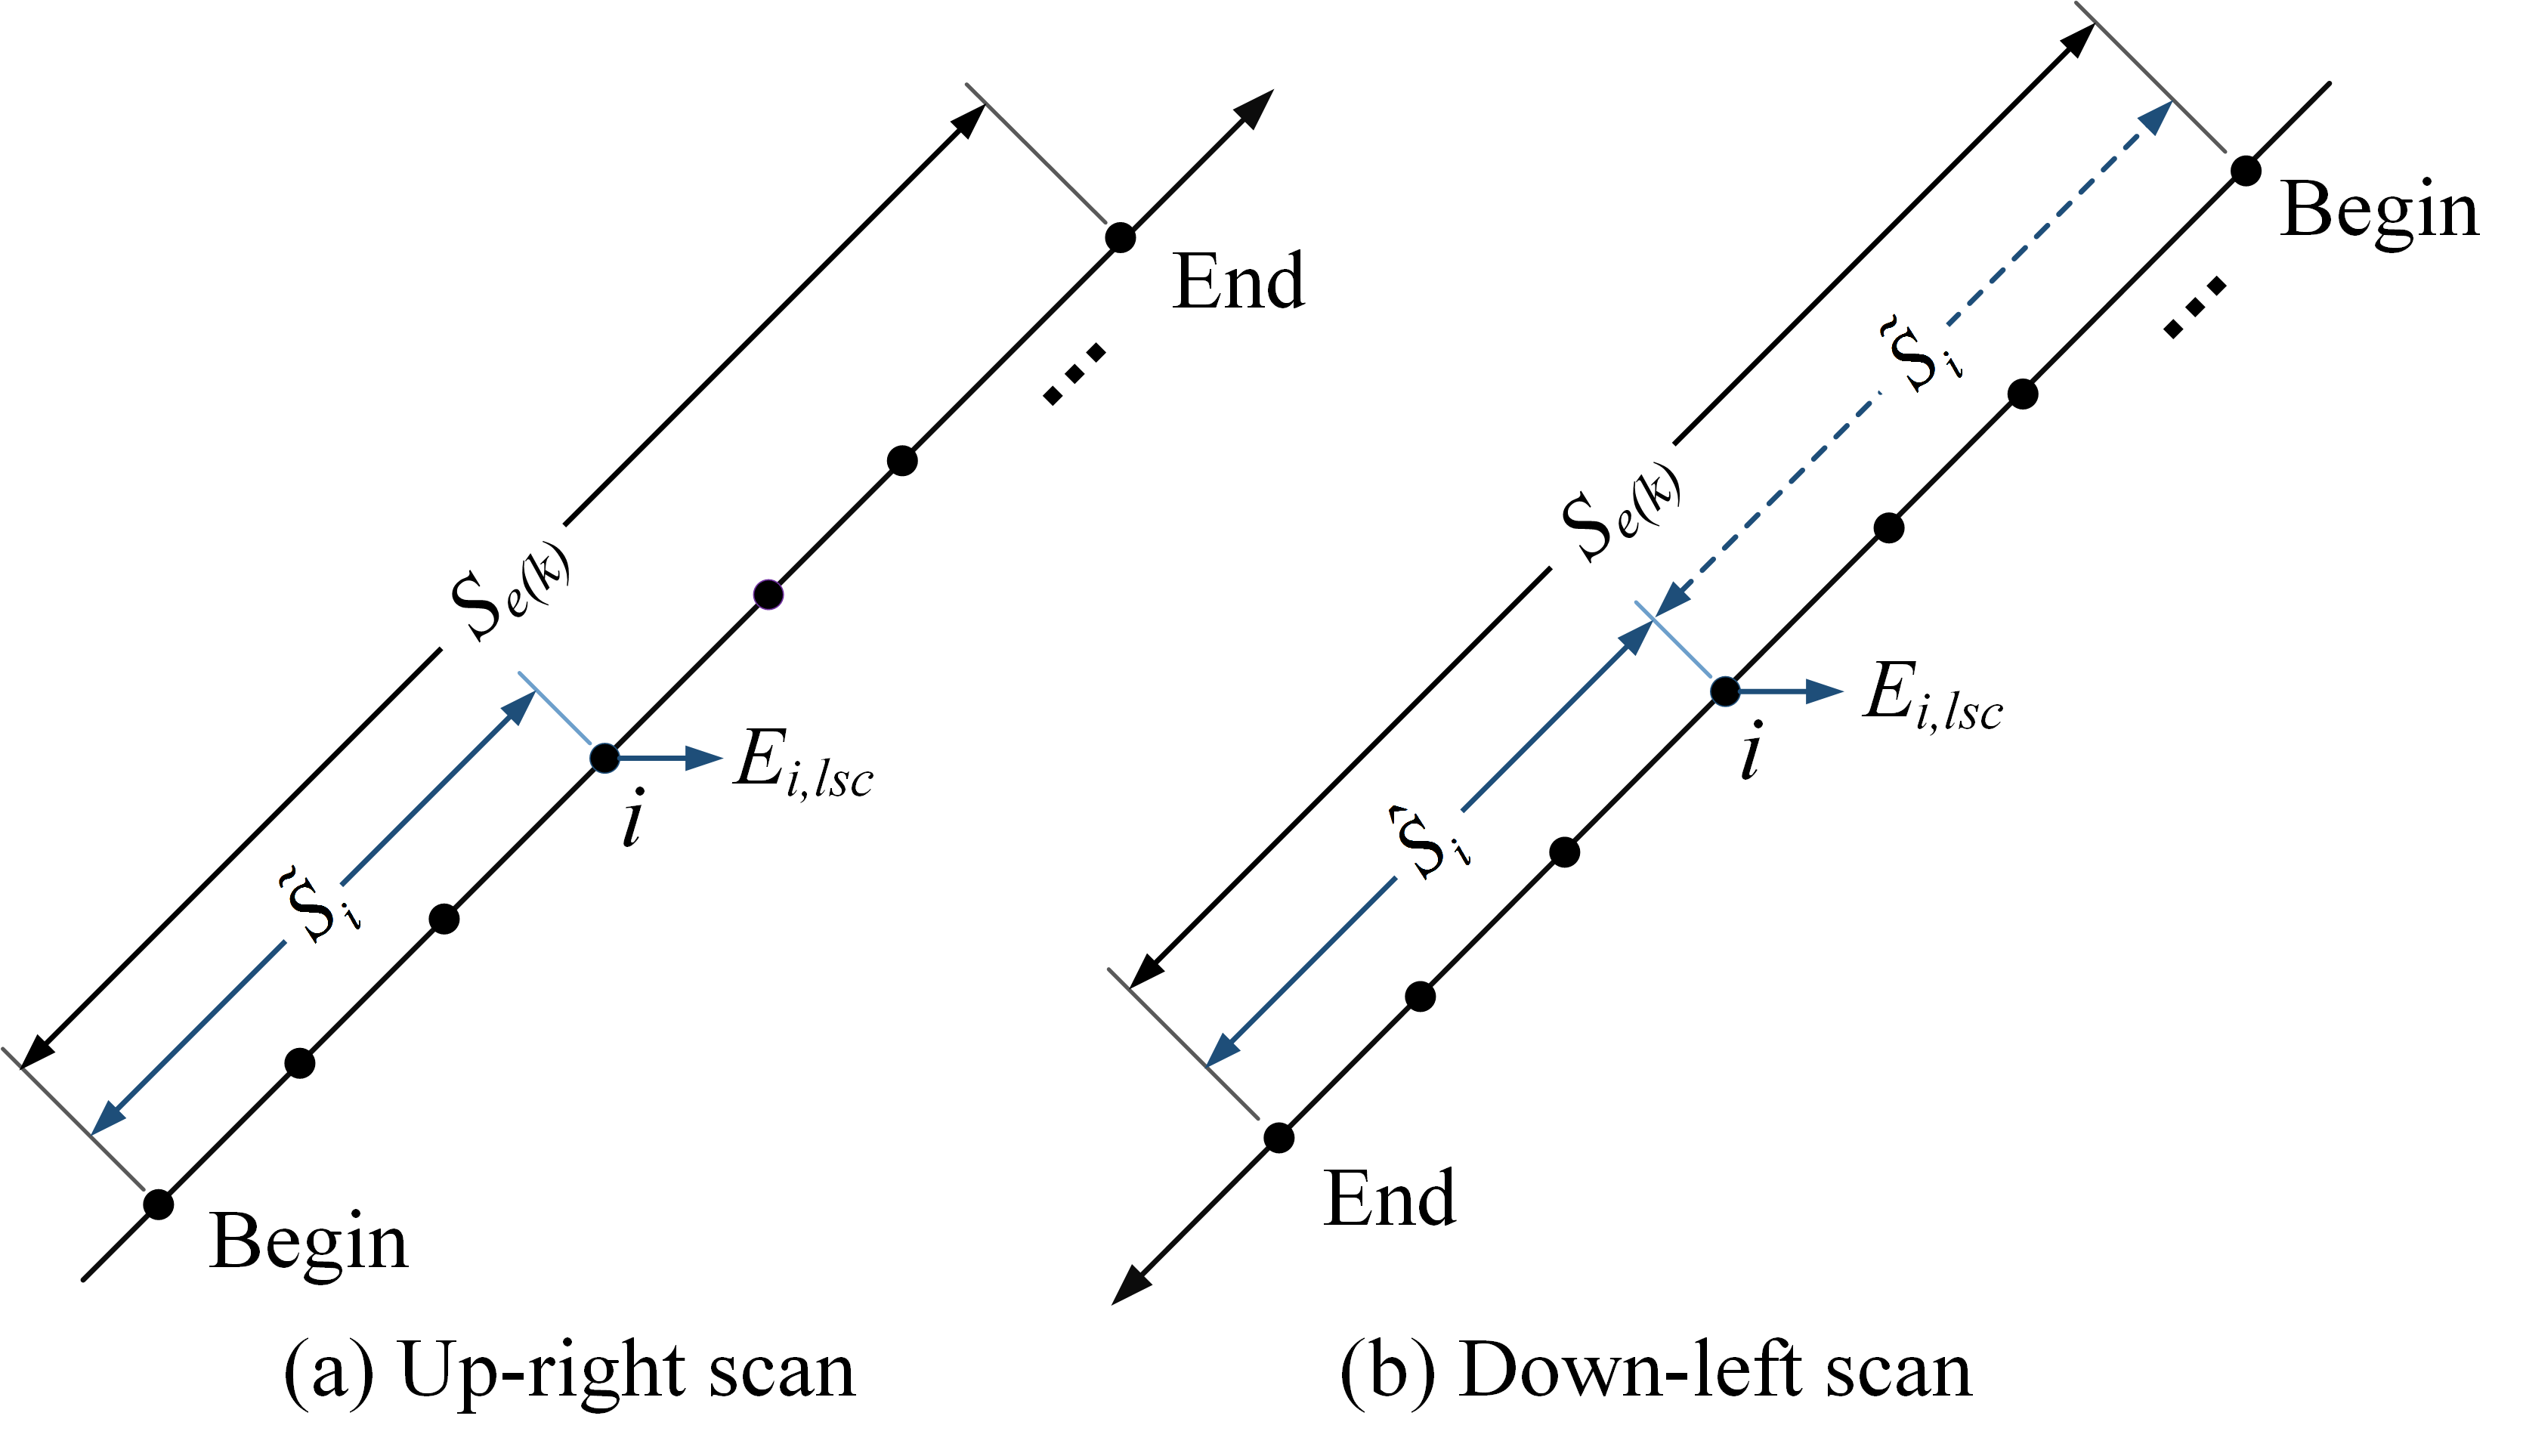
\includegraphics[width=0.49\textwidth]{figure/abcompare.png}} 
	% figure caption is below the figure
	\caption{The illustration of the accumulated cost variables $S$.}
	\label{abcompare} % Give a unique label
\end{figure}
\par
\begin{figure}[!ht]
	\centering
	\centerline{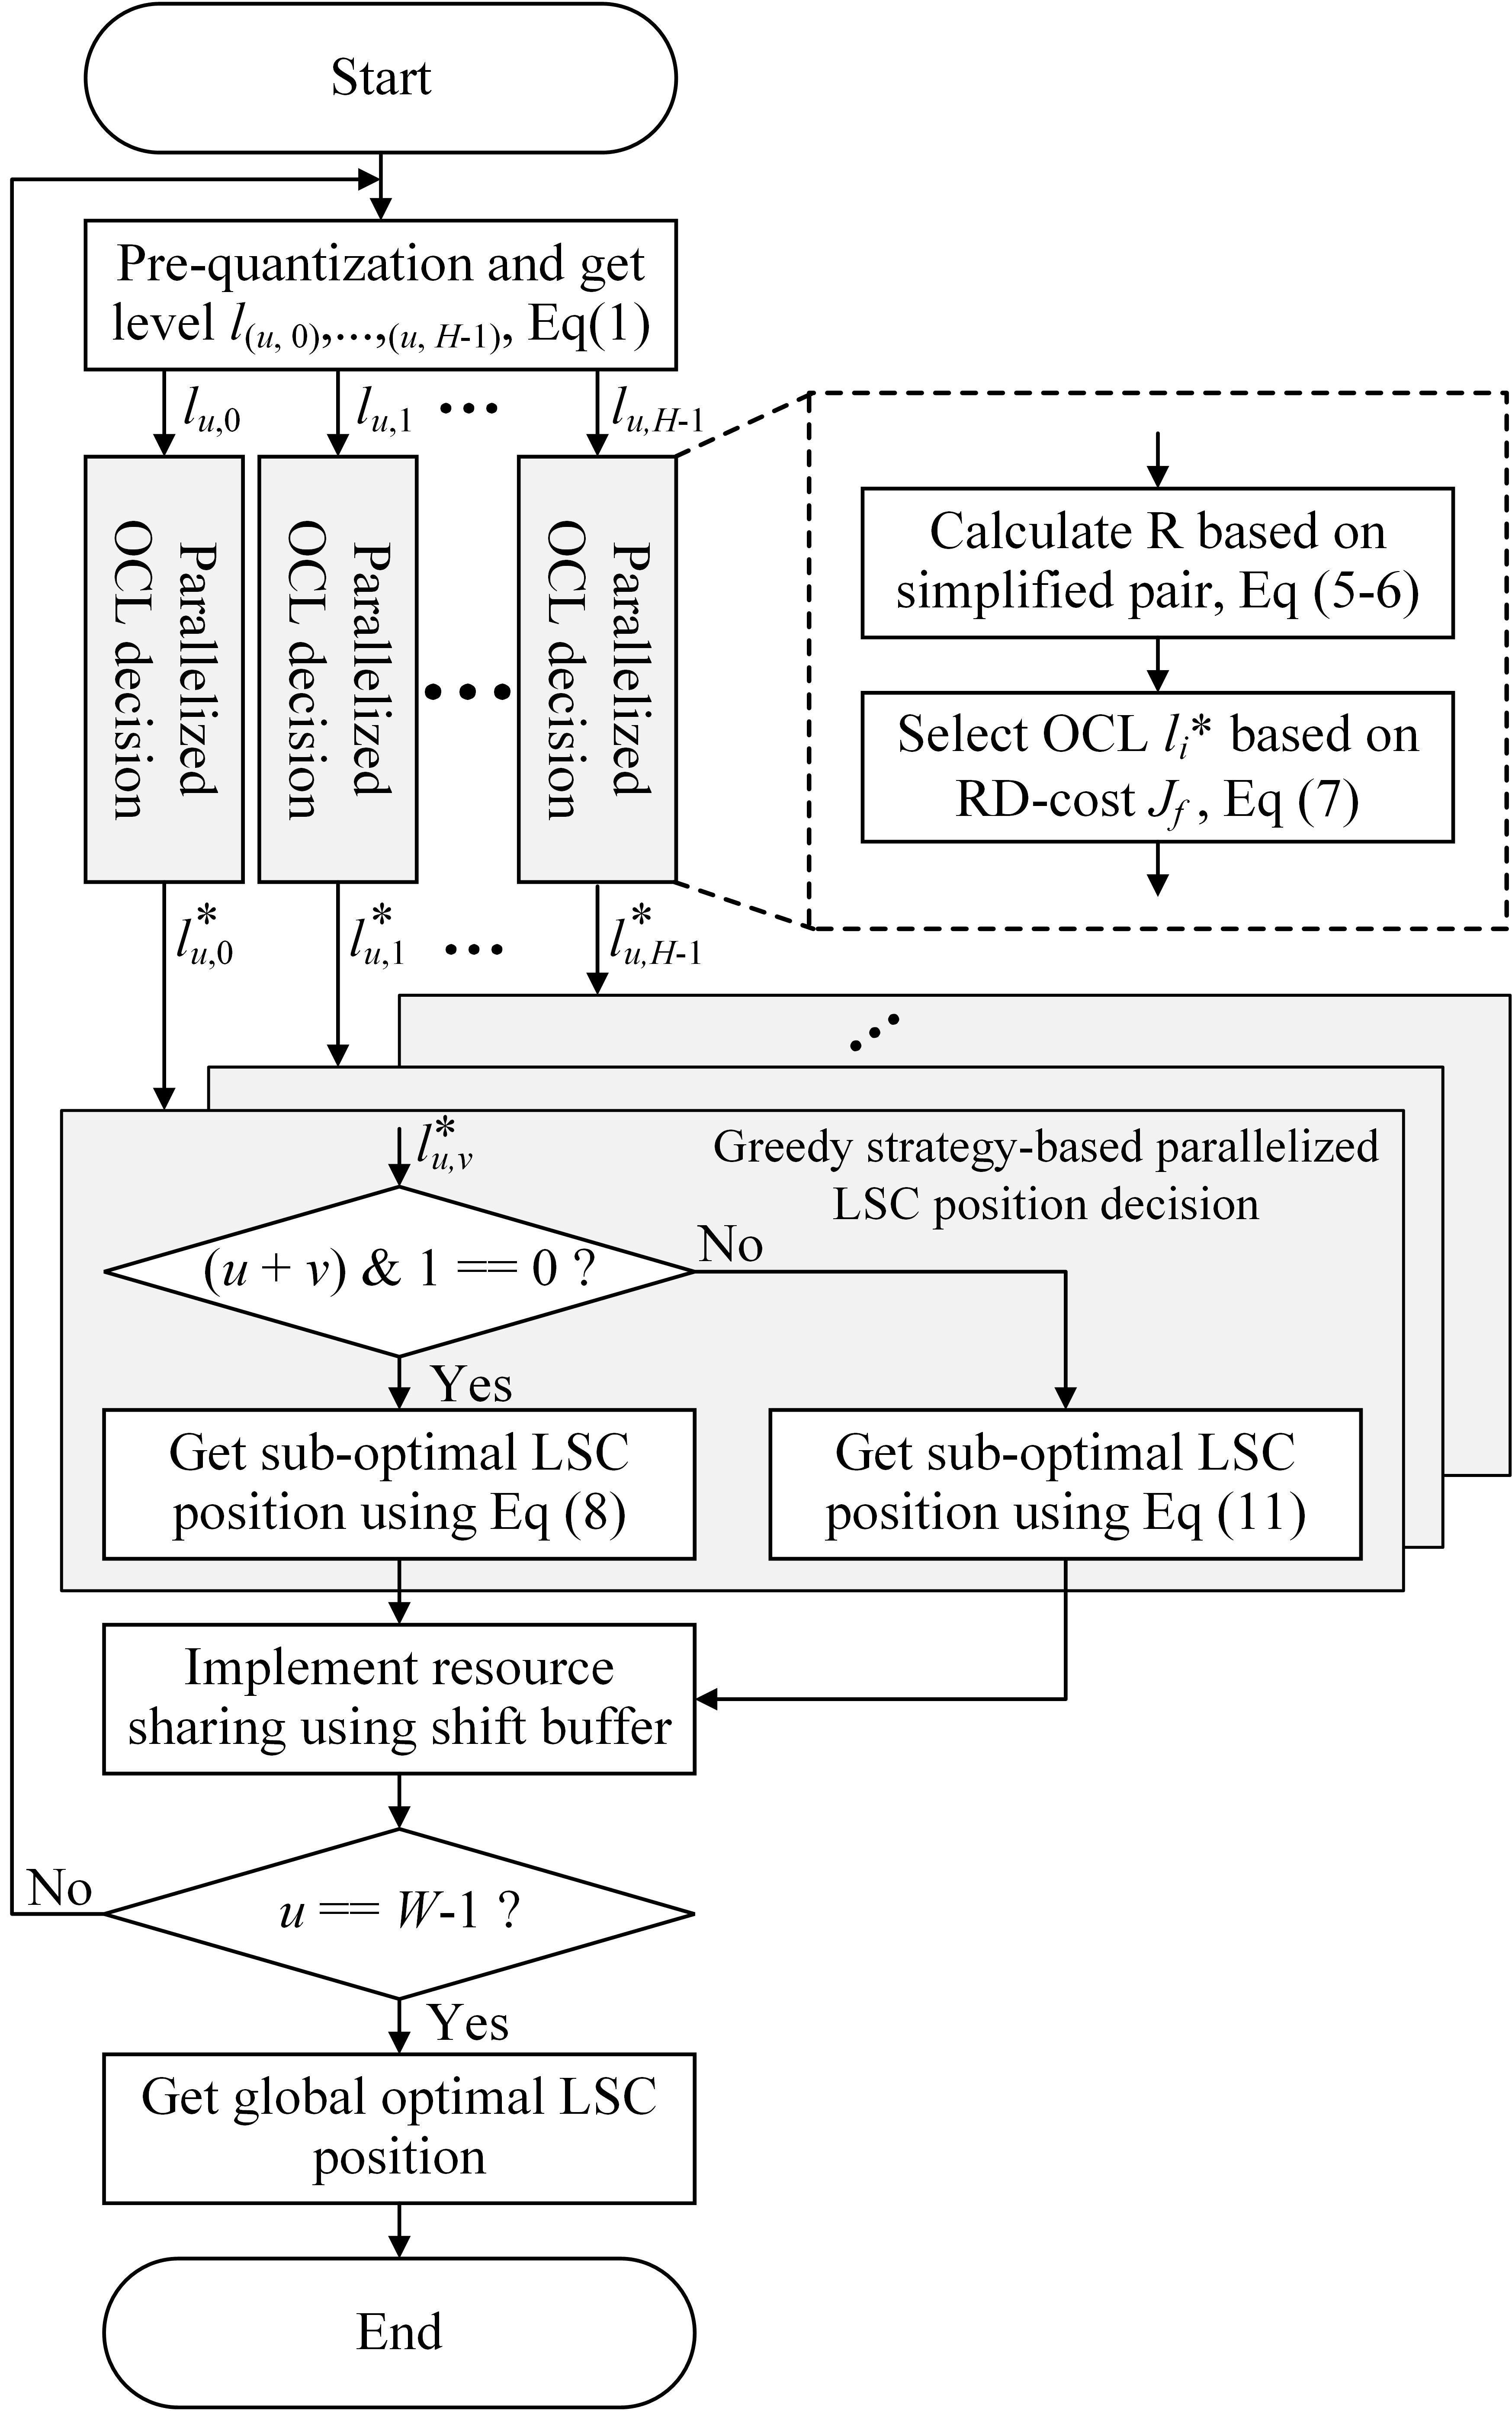
\includegraphics[width=0.48\textwidth]{figure/ProRDOQ.png}} 
	% figure caption is below the figure
	\caption{The flowchart of the proposed parallelized RDOQ algorithm.}
	\label{ProRDOQ} % Give a unique label
\end{figure}
For the optimal $i^{*}$ derived based on Eq.~\eqref{li_to_lk}, it will need to buffer all suboptimal $i_{k}^{*}$ and then compare their accumulated cost to decide the best. Since there are a total of $W+H-1$ scanlines, this means that it will need to buffer $W+H-1$ times resources. To save the buffer, an on-the-fly decision approach is proposed. When the LSC position decision processes the coefficients at column $u$, the $i^{*}$ for all previous $u-1$ scanlines is derived simultaneously. The accumulated cost for the optimal $i_{u-1}^{*}$ can be calculated using Eq.~\eqref{ur_compare}. Then, the optimal $i^{*}$ for all $u-1$ scanlines can be derived by comparing with the minimum accumulated cost. It is noted that the remaining $H-1$ scanlines should be added to the comparison when all $W$ scanlines finish the on-the-fly process. With this optimization, it will need to only buffer $H$ times resources. The $H$ times resources are shared by all $W+H-1$ scanlines and are implemented using a shift buffer. 
\begin{equation}
	\begin{aligned}
	\label{ur_compare}
	J_{i_{u-1 }^{*}} = \left ( \sum_{j=0}^{u-2} \widetilde{S}_{e(k)} + \widetilde{S}_{i_{u-1 }^{*}} + E_{i_{u-1 }^{*},lsc}   \right) 
\end{aligned}
\end{equation}
\subsection{Proposed parallelized RDOQ algorithm}
\label{subsec:paraRDOQ}
As described previously, we propose a parallel RDOQ scheme that consists of two components: a parallel OCL decision and a greedy strategy-based parallel LSC position decision. An overview of the flowchart is shown in Fig.~\ref{ProRDOQ}. In the parallel OCL decision, we calculate the simplified ($run$, $prev\_level$) pair to remove partial dependency for rate estimation and propose an efficient RD cost form $J_{f}$ to reduce rate cost computation and save chip area. In the greedy strategy-based parallel LSC position decision, the optimal $i^{*}$ is derived based on the suboptimal $i_{k}^{*}$ for each scanline $k$, where the derivation of $i_{k}^{*}$ can be executed in parallel for each scanline. Moreover, a shift buffer is utilized to save the buffer. With these optimizations, the scan order of the RDOQ can be changed from zig-zag order to column-first order, which aligns with the output of DCT. The data dependency only exists within the scanline, which means that all coefficients in the same column can be processed in parallel. This is illustrated in Fig.~\ref{zig2col}. We provide a detailed description of the proposed parallelized RDOQ algorithm in Algorithm \ref{the proposed LNPD algorithm}. 
\begin{figure}[!h]
	\centering
	\centerline{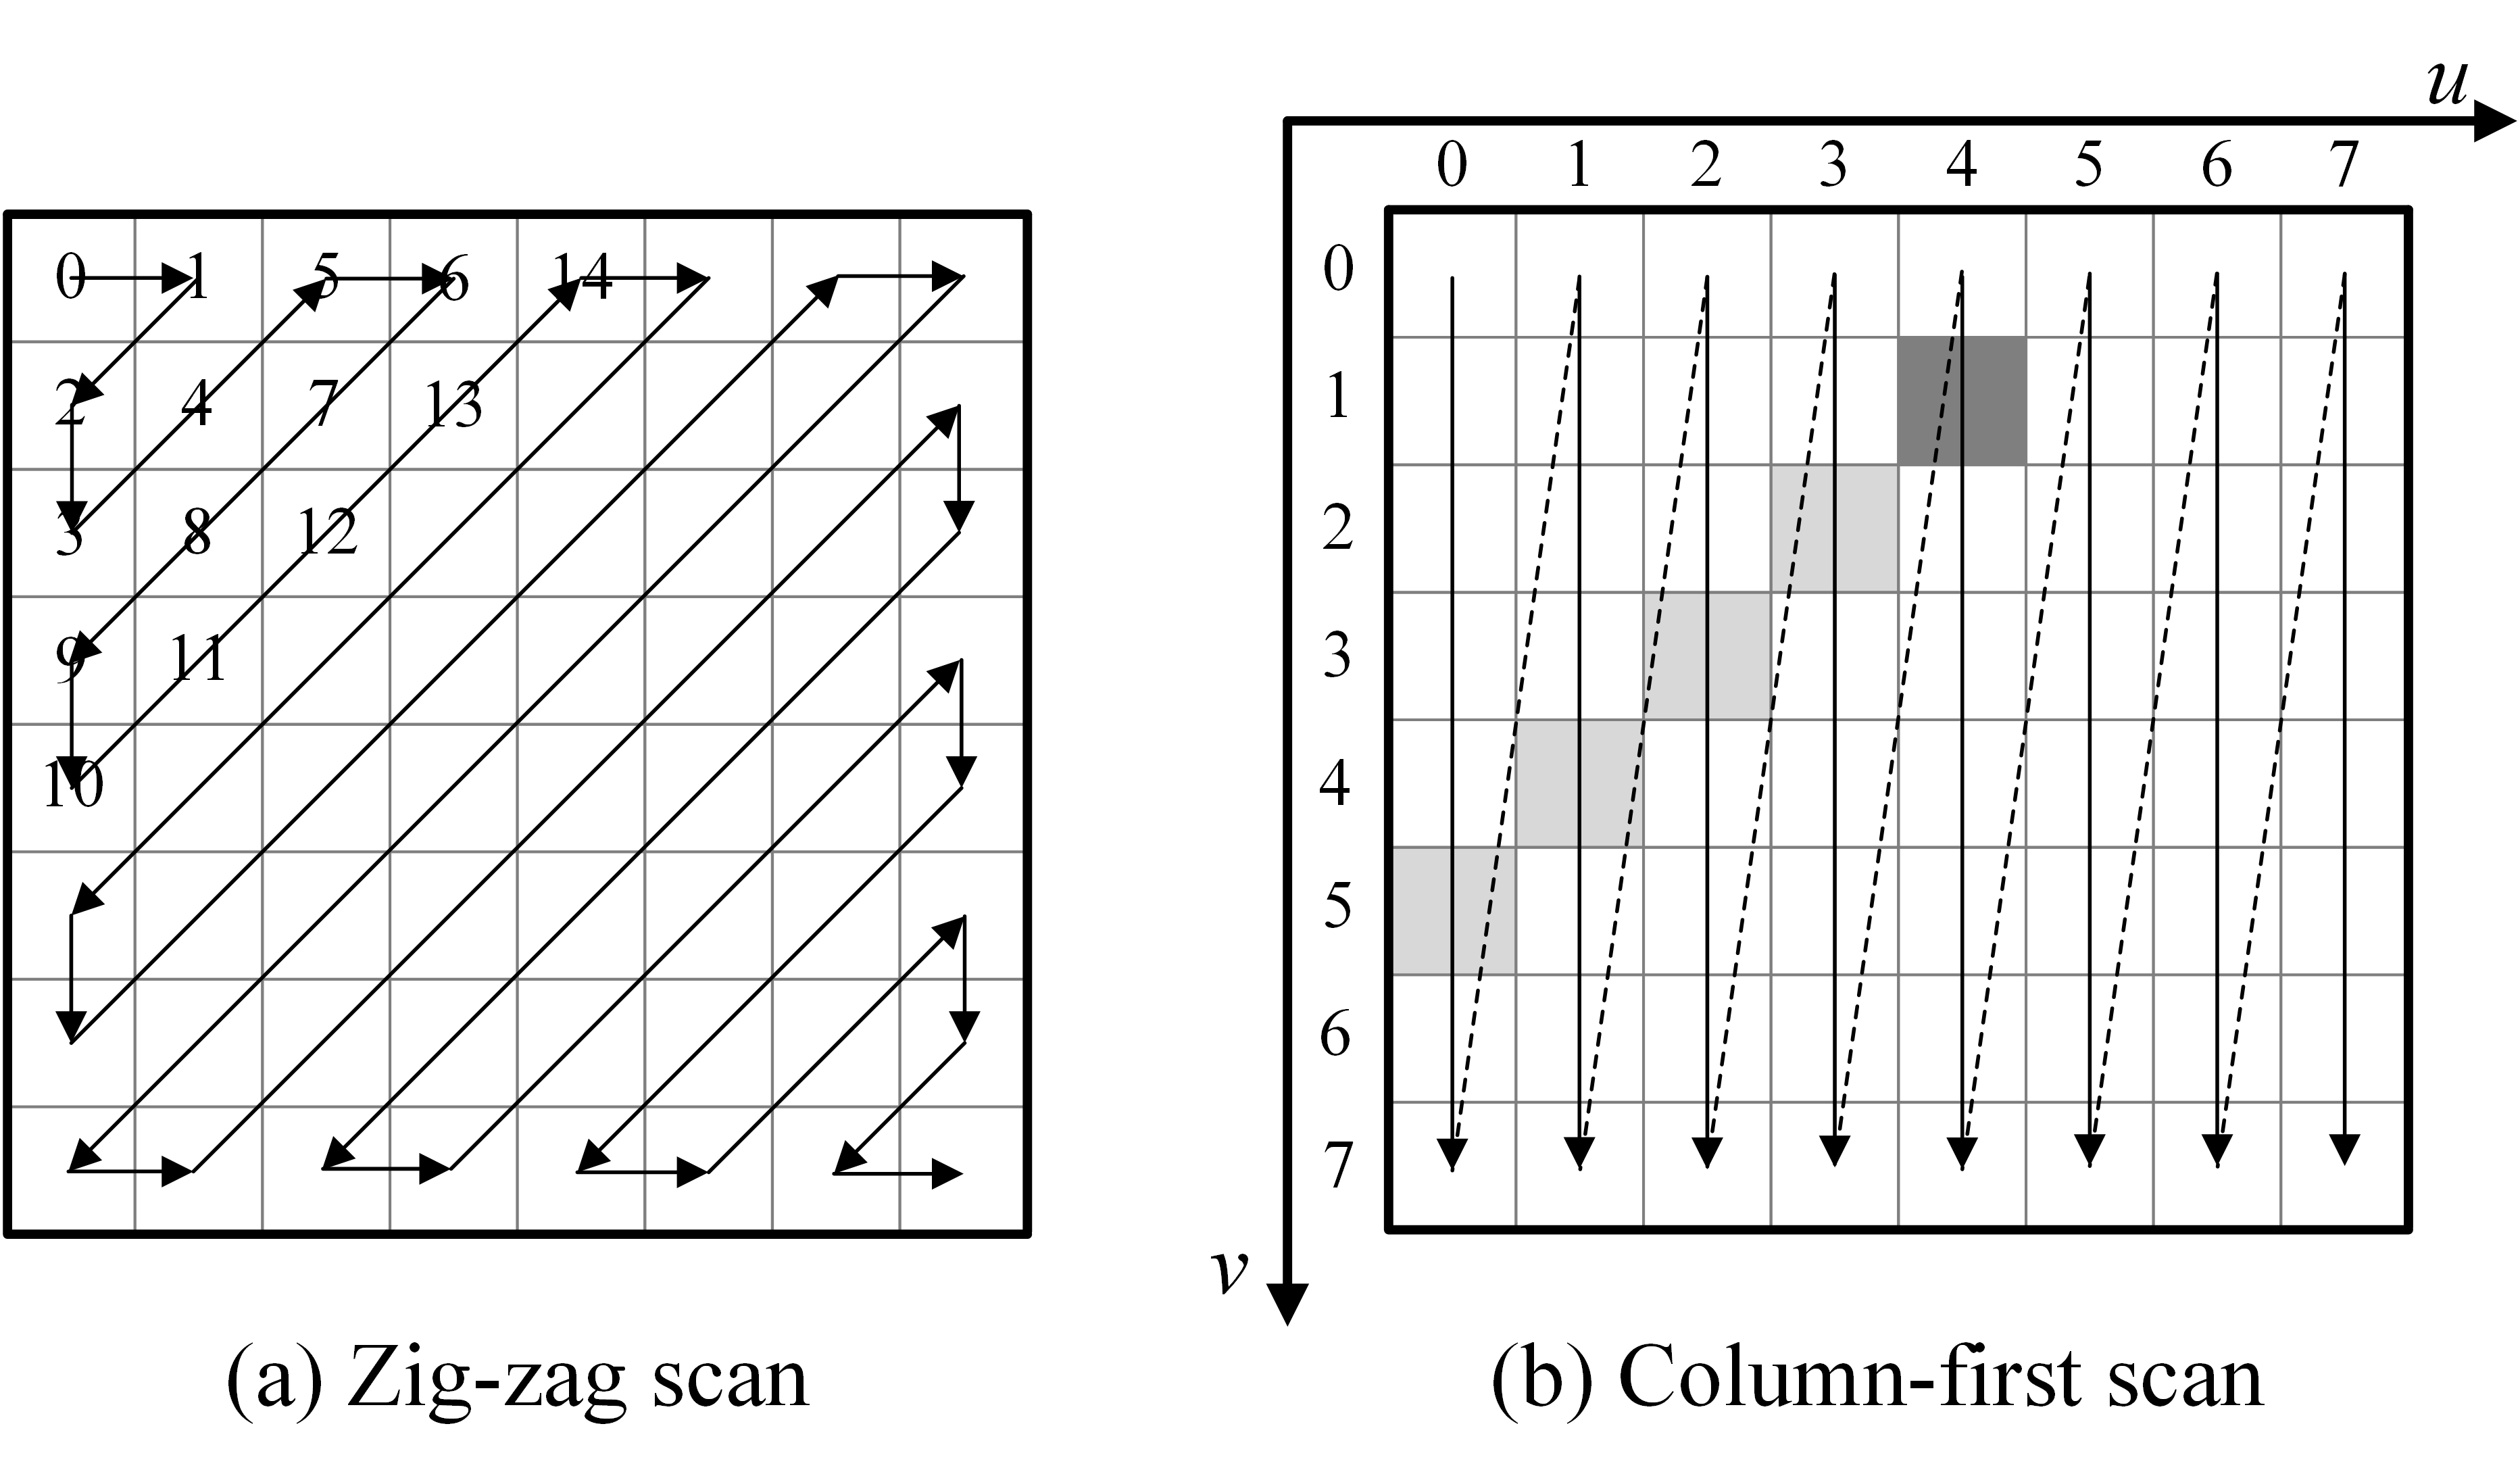
\includegraphics[width=0.49\textwidth]{figure/zig2col.png}} 
	% figure caption is below the figure
	\caption{Diagram of the scan order conversion from (a) zig-zag order to (b) column-first order. In (b), the dark gray coefficient depends on the previous light gray coefficients in the inner zig-zag scanline.}
	\label{zig2col} % Give a unique label
\end{figure}

\begin{algorithm}[!ht]
  \renewcommand{\algorithmicrequire}{\textbf{Input:}}
  \renewcommand{\algorithmicensure}{\textbf{Output:}}
  \caption{The proposed parallelized RDOQ algorithm}
  \label{the proposed LNPD algorithm}
	\begin{algorithmic}[1] 
	\REQUIRE  $c_{0,..,W \times H-1}$, \ $W$, \ $H$, \ $\lambda$.      
	\ENSURE $l_{0,..,W \times H-1}^{*}$, \ $i_{}^{*}$. \\      
	\STATE $\textsc{Temp \ buffer:} \ S_{best}[H], \ E_{best}[H], \ S_{all}[H], \ i_{best}^{*}[H]$;
	% for loop1
	\FORALL {$u = 0,1,\cdots,W-1$}
	% for loop2
	\FORALL {$v = 0,1,\cdots,H-1$}
	\STATE Get $c_{i}$, zig-zag index $i$ is derived based on ($u$, $v$);
	\STATE Calculate $l_{i}$ based on Eq.~\eqref{round};
	\STATE Calculate $prev\_level_{i}$ and $run_{i}$ based on Eq.~\eqref{prevlevel} and Eq.~\eqref{run}, respectively;
	\STATE Calculate $R$, where $R$ = $f$\;($prev\_level_{i}$, $run_{i}$, $l_{i}$);
	\STATE Get optimal level $l_{i}^{*}$ by $ \mathop{\arg\min}\limits_{ L_{i} } \left ( J_{f} \right) $.

	\IF { $u==0$ or $v==W-1$ }
		\STATE Initial: $\widetilde{S}_{best}[v] \gets \Delta J_{v}$, ${E}_{best}[v] \gets E_{v,lsc}$, ${S}_{all}[v] \gets 0$, $i_{best}^{*}[v] \gets i$;
	\ELSE
		\IF { $(u + v) \ \& \ 1$ } 
		    \STATE $\hat{S}_{i}$ = ${S}_{all}[v]$ +  $\Delta{J}_{v}$;\ // down-left scanline
		    \IF{$-\hat{S}_{i}$ + $E_{i,lsc}$ $<$ $-{S}_{best}[v]$ + $E_{best}[v]$}
	    	\STATE ${S}_{best}[v] \gets \hat{S}_{i}$, ${E}_{best}[v] \gets {E}_{i,lsc}$, \\ $i_{best}^{*}[v] \gets i$;
		    \ENDIF
		    \STATE ${S}_{all}[v] \gets \hat{S}_{i}$;
		\ELSE 
	    	\STATE $\widetilde{S}_{i}$ = ${S}_{all}[v]$ + $\Delta{J}_{v}$; \ // up-right scanline
	    	\IF{$\widetilde{S}_{i}$ + $E_{i,lsc}$ $<$ ${S}_{best}[v]$ + $E_{best}[v]$}
	    	\STATE ${S}_{best}[v] \gets \widetilde{S}_{i}$, ${E}_{best}[v] \gets {E}_{i,lsc}$, \\ $i_{best}^{*}[v] \gets i$;
	    	\ENDIF
	    	\STATE ${S}_{all}[v] \gets \widetilde{S}_{i}$;
		\ENDIF
	\ENDIF
	
	\ENDFOR       % end loop2
	\STATE Select the optimal $i_{}^{*}$ for $u$ scanlines according to Eq.(12);
	
	\FORALL {$v = 1,2\cdots,H$}
	\STATE Implement resource sharing using shift buffer: ${S}_{best}[v-1] \gets {S}_{best}[v]$, ${E}_{best}[v-1] \gets {E}_{best}[v]$, ${S}_{all}[v-1] \gets {S}_{all}[v]$, ${i}_{best}^{*}[v-1] \gets {i}_{best}^{*}[v]$;
	\ENDFOR
	
	\ENDFOR       % end loop1

	\FORALL {$t = 1,2,\cdots,H-1$}
	\STATE Compare the remaining cost to determine the global optimal $i_{}^{*}$;
	\ENDFOR
	%\STATE \textbf{return} $\mathbf{Pos}$
	\end{algorithmic}
\end{algorithm}


\subsection{SIMD-based fast RDOQ} 
Although the algorithm proposed in subsection \ref{subsec:paraRDOQ} can be run in parallel for all coefficients within the same column, it may take longer execution time on the Intel X86 platform as each coefficient is processed without skipping. A SIMD-based approach is adopted to address this issue, and the implementation and design are explained below. 


During the pre-quantization step, each transform coefficient is processed independently. In the SIMD optimization, we execute four coefficients simultaneously by utilizing intrinsics. Similarly, the parallelism is four coefficients per instruction in the OCL decision step, consistent with the parallelism of the pre-quantization step. For the decision of $l_{i}^{*}$, there may have different numbers of candidate level $L_{i}$ for each of the four parallelized coefficients, which will impact the parallelization by intrinsic due to its irregularity. To address this issue, all coefficients will calculate the RD cost for three candidate levels as shown in Fig.~\ref{selection}. It should be noted that the candidate levels for the gray color block will not participate into the optimal level $l_{i}^{*}$ comparison. For the intrinsic of minimum cost comparison, the PCMPGTD instruction is used and the result is bit-inverted by the VPANDN instruction.

%\par
\begin{figure}[!h]
	\centering
	\centerline{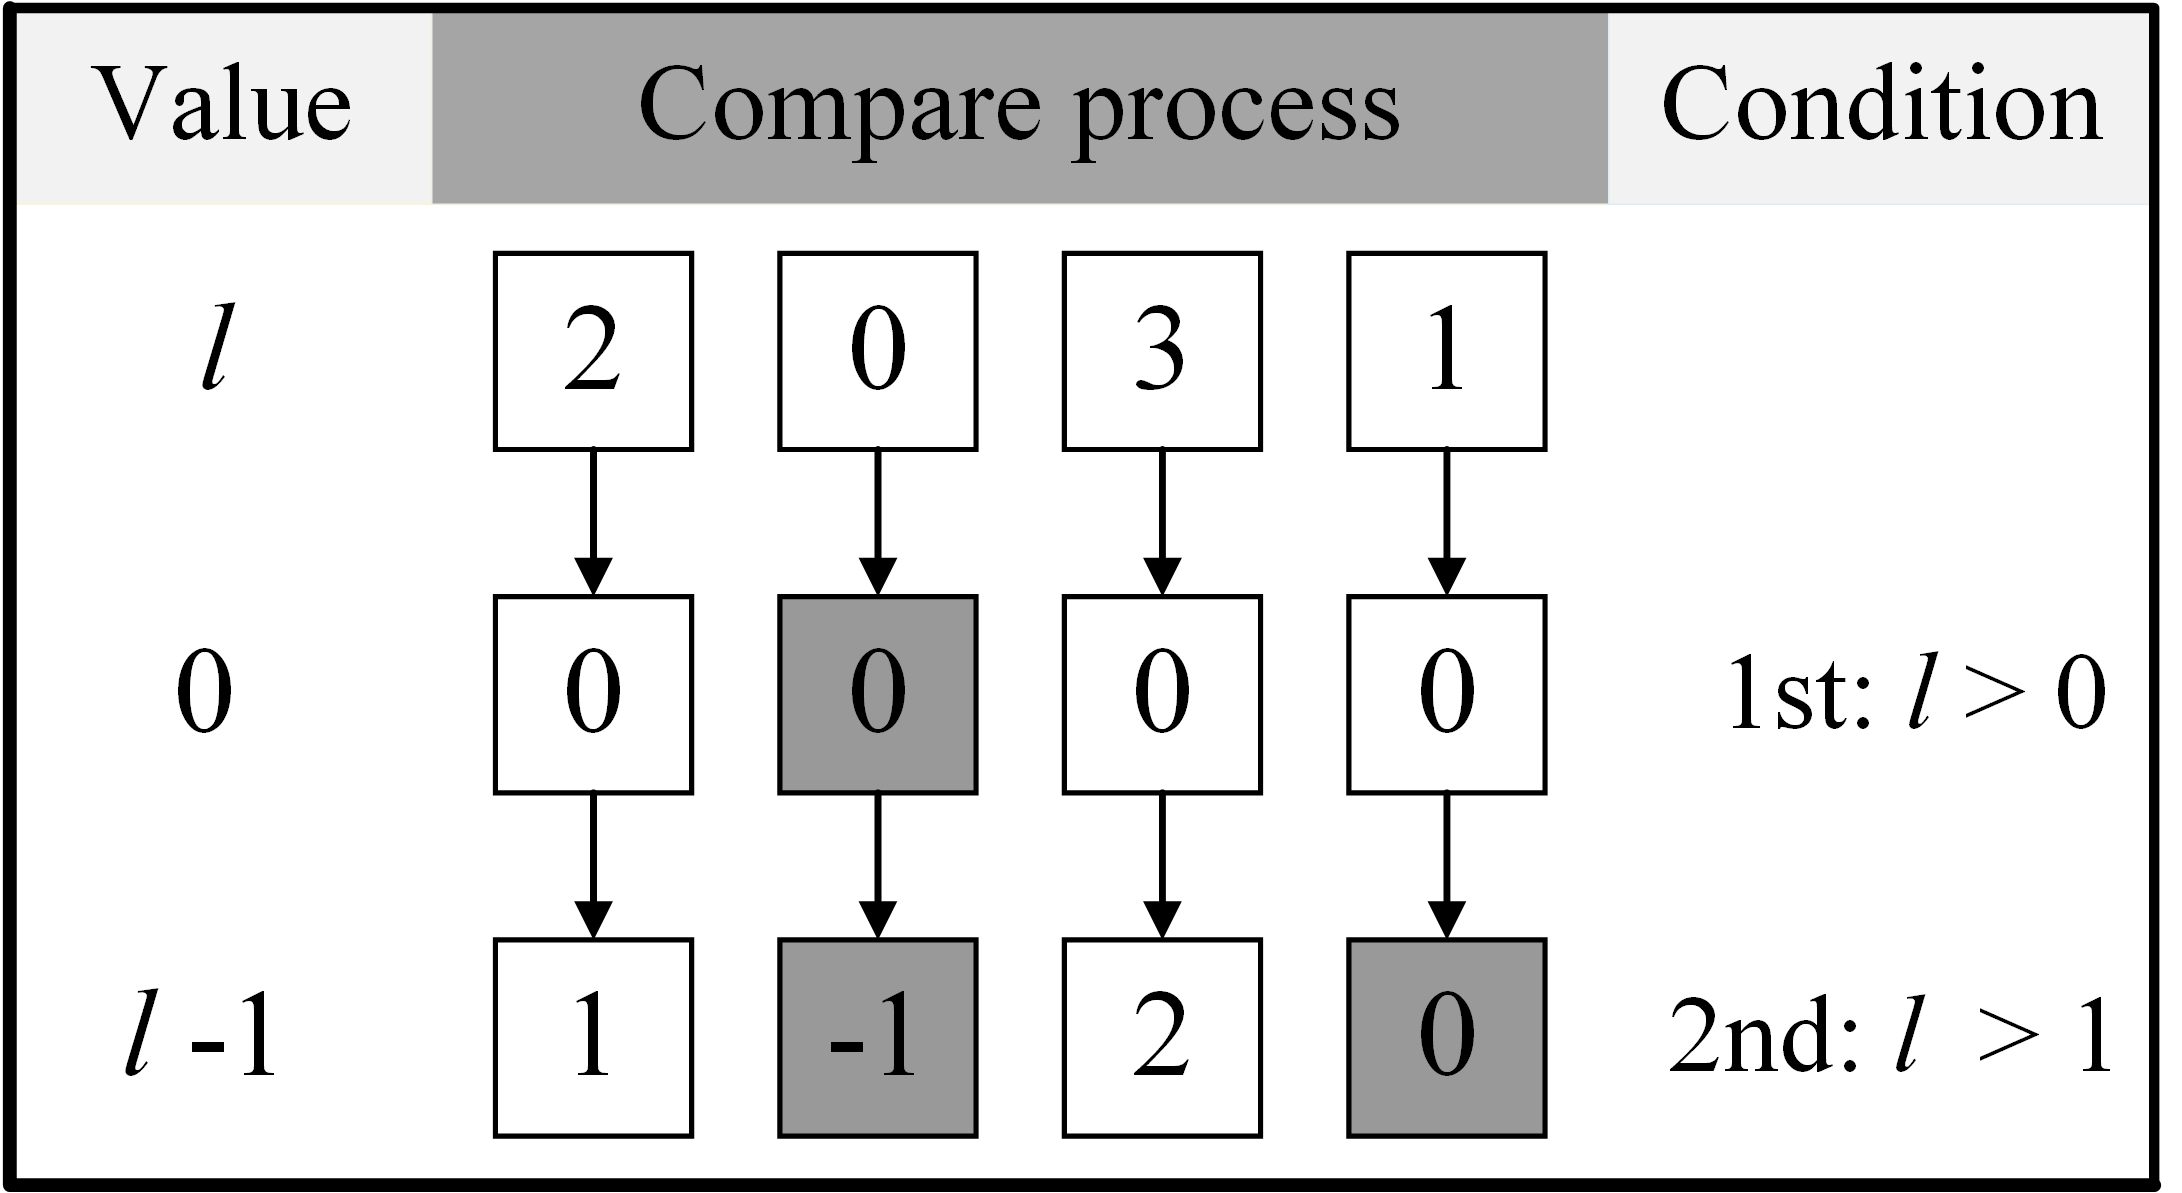
\includegraphics[width=0.38\textwidth]{figure/SIMDSEL.png}} 
	% figure caption is below the figure
	\caption{An example of OCL decision process using SIMD.}
	\label{selection} % Give a unique label
\end{figure} 

In the LSC position decision step, the pixel parallelism is four coefficients similar to the previous steps. The shift buffer is adopted to save the buffer as illustrated in subsection \ref{subsecgreedy}. Rotation instruction is needed to implement this behavior. We use the VPSRLDQ, Extract, and Insert operations to rotate the data. VPSRLDQ instruction shifts the data in the 128-bit channel by a specified byte, the extract operation extracts the data in the channel, and the insert operation inserts the data into a specified location, respectively. 

\section{Fully pipelined Hardware Architecture Design}
It is a fact that the RDOQ algorithm shows high computational complexity and strong data dependency, which poses significant challenges for real-time video coding. In the previous section \ref{sec:3}, a parallelized RDOQ algorithm is proposed to resolve these problems. In this section, a fully pipelined and high-throughput hardware architecture is designed for the parallelized algorithm. 
\par
\begin{figure*}[htbp]
	\centering
	\centerline{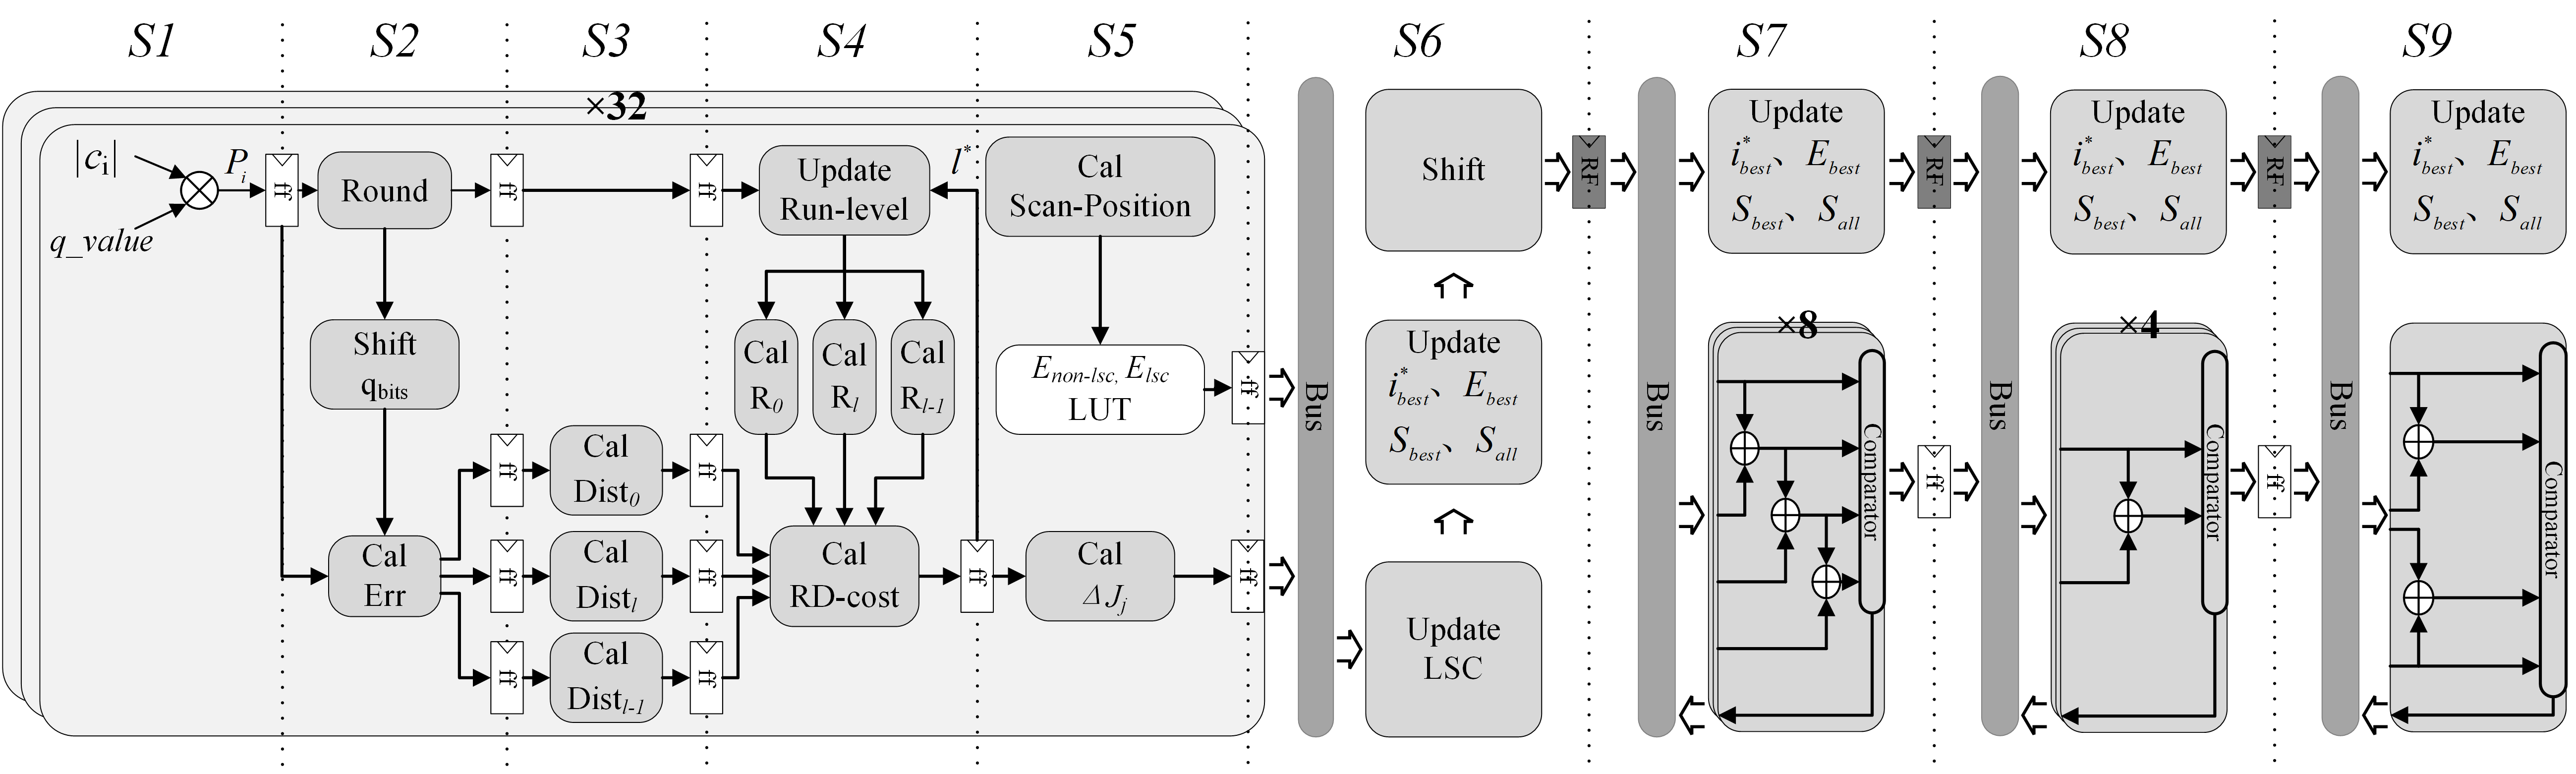
\includegraphics[width=0.90\textwidth]{pic_pan/overall_architecture.png}} 
	% figure caption is below the figure
	\caption{The hardware architecture design of the parallelized RDOQ algorithm.}
	\label{timing diagram} % Give a unique label
\end{figure*}

\subsection{Overall Architecture}
The TU size in AVS3 standard can range from $4\times4$ to $64\times64$. However, to reduce the coefficient coding for large TU size, only the first 32 rows/columns coefficients are kept and the high-frequency coefficients are zeroed out. As a result, the width $W$ and height $H$ of the TU for RDOQ must not exceed 32. To facilitate this constraint, the RDOQ hardware architecture is designed with a pixel parallelism of 32, which means that a maximum of 32 coefficients within the same column can be processed simultaneously. To improve parallelism for TUs with height $H$ smaller than 32, multiple TUs are combined and processed in parallel by reusing hardware resources. Specifically, the architecture can simultaneously process eight $W\times4$ TUs, four $W\times8$ TUs, and two $W\times16$ TUs, respectively. The width $W$ should be uniform across the parallelized TUs. 

The designed hardware architecture is shown in Fig.~\ref{timing diagram}. The architecture consists of nine pipeline stages, where the pre-quantization step occupies $S1$ and $S2$, the OCL decision step occupies $S2$, $S3$, and $S4$, and the LSC decision step occupies the last five pipeline stages. From $S1$ to $S6$, it will be on-the-fly processing for each column, which implements the for loop from line 2 to 31 in Algorithm \ref{the proposed LNPD algorithm}. From $S7$ to $S9$, it decides the final optimal $i_{}^{*}$, which implements the for loop from line 32 to 34 in Algorithm \ref{the proposed LNPD algorithm}. The four-input sequential comparator is adopted to get the optimal $i_{}^{*}$. As the maximum $H$ is 32, $S7$ utilized eight comparators, $S8$ utilized two comparators, and $S9$ utilized one comparator, respectively. 

The timing diagram xxx. plot different TUs, Wx4 Wx8 Wx16 Wx32 cases. ... 

\subsection{Pre-quantization}
In the pre-quantization step, all the transform coefficients $c_{i}$ undergo the absolute, multiplication, and round operations according to Eq.~\eqref{round}. The division operation in Eq.~\eqref{round} is transformed to multiplication and shift operations in HPM-4.0.1. The equation is shown as follow,

\begin{equation}\label{Qp}
	\begin{aligned}
		P_{i} = \lvert c_{i} \rvert \times q_{value},
	\end{aligned}
\end{equation}

\begin{equation}\label{l}
	\begin{aligned}
		l = round \left ( P_{i} \right ) >> q_{bits},
	\end{aligned}
\end{equation}
where $q_{value}$ is derived according to $QP$ and TU size, $c_{i}$ is the transform coefficient, $q_{bits}$ is the shift precision, $P_{i}$ is the multiplication result at stage $S1$, $l$ is the initial scalar quantization level.

It is obvious that there is no data dependency in this step, all coefficients output from different TUs can be processed in parallel. The hardware architecture is shown as $S1$ and $S2$ in Fig.~\ref{timing diagram}. 

\subsection{OCL decision}

The strong run-level context dependency between neighboring coefficients poses a challenge for parallelized OCL hardware implementation and hinders real-time processing. However, this data dependency problem is partially resolved by the parallelized OCL algorithm in subsection \ref{subsecOCL:B}. 
The proposed algorithm segregates the context dependency from TU-level to zig-zag scanline line level, which makes the data dependency exist within one scanline. The scanline-level dependency exists for the derivation of the variables $pre\_level_i$ and $run_i$, and their derivation process is shown in Eq.~\eqref{prevlevel} and Eq.~\eqref{run}. From these two formulas, it indicates that the $pre\_level_i$ and $run_i$ depend on the optimal coefficient level $l _{i-1}^{*}$ or $l _{i+1}^{*}$ for the up-right and down-left scanline, respectively. However, determining the optimal coefficient level involves complex RD cost calculations, in which the rate cost, in turn, depends on $pre\_level_i$ and $run_i$. 

As a result, this dependency increases the complexity of the hardware design. To resolve the above problem, the $pre\_level_i$ and $run_i$ derivation and optimal coefficient level decision are implemented in a single cycle, and then utilizing data-forwarding method to resolve this dependency \cite{harris2010digital}. 
Furthermore, to improve the timing of the design, the RD cost calculation is divided into three distinct pipeline stages, spanning from $S2$ to $S4$. 
The pipeline stage for distortion calculation is allocated prior to the rate calculation, spanning from $S2$ to $S3$, while the rate calculation and RD cost comparison are scheduled at stage $S4$. This is because the distortion is calculated without context dependency for all candidate levels.

Considering that the maximum number of candidate levels would not surpass three as listed in Tab.~\ref{tab:candidate list}, the rate calculation architectures and the distortion calcualtion architectures are instantiated in parallel for three distinct candidates. As shown in Fig.~\ref{timing diagram}, where $Dist_{0}\&R_{0}$, $Dist_{l-1}\&R_{l-1}$ and $Dist_{l}\&R_{l}$ represent the distortion cost and rate cost of different candidates. 

Following the optimization of the RD cost calculation mentioned in equation \ref{pRDcost}, the calculation of distortion is determined by the following formula,

\begin{equation}\label{err}
	\left\{
		\begin{aligned}
			&Err_{0} 	=  P_{i} \times S_f >> 20,  \\
			&Err_{l-1} 	= \left ( P_{i} - \left ( \lvert l-1 \rvert << q_{bits} \right ) \right ) \times S_f >> 20,  \\
			&Err_{l} 	= \left ( P_{i} - \left ( \lvert l \rvert << q_{bits} \right ) \right ) \times S_f >> 20,  \\ 
		\end{aligned}
	\right.
\end{equation}

\begin{equation}\label{distortion}
	\begin{aligned}
		Dist_{j} = Err_{j}^{2}, j = 0, l-1, l,
	\end{aligned}
\end{equation}
where $q_{bits}$ is the shift precision, $P_{i}$ is the multiplication result at stage $S1$, $l$ is the initial scalar quantization level, $j$ is the value of the candidates of the optimal quantization level, $S_f$ is the scaling factor with the $lambda$ optimization in subsection \ref{subsecOCL:B}. To improve timing performance, the distortion calculation is distributed from stage $S2$ to $S3$, where each stage has a multiplication operation.

Due to that the RD cost is optimized to a more efficient form in subsection \ref{subsecOCL:B}, there is no multiplication operation in pipeline stage $S4$. The calculation of $R_{0}$ is relatively simple, enabling direct access. Additionally, the rate calculation architecture for $R_{l}$ and $R_{l-1}$ is divided into three datapaths, as shown in Fig.~\ref{rate cost}. 
In this figure, table $est\_level$ is derived from entropy coding, $ctx\_level$ represents the minimum value between $pre\_level_i$ and 5, $L$ is the value of the candidate.

When $L$ is equal to one, the rate cost is derived from table $est\_level$ indexed by $ctx\_level$. 
For values of $L$ greater than eight, the rate cost calculation becomes more intricate. 
In addition to considering the lookup value from table $est_level$, it also takes into account the Golomb coding of $L-9$. 
For the remaining value of the candidates, the rate cost also depends on the lookup value from the table $est\_level$. Furthermore, an integral component of the rate cost calculation involves multiplying the lookup value with the value of $L$. All multiplication operations involving $est\_level$ and the limited range of candidates (between one and eight) are implemented using separate add and shift operations, thus reduce the area consumption and benefit the timing greatly. 

As mentioned earlier, the calculation of rate cost and the comparison of RD-cost are executed within a single cycle due to the context dependency. Once all rate costs have been calculated, the minimum RD-cost is identified and selected as the optimal choice. The corresponding candidate is then designated as the optimal coefficient level $l_{i}^{*}$. Subsequently, this optimal coefficient level is transmitted back to update the run-level.

%%%%%%%%%%%%%%%%%%%
\begin{figure}[!h]
	\centering
	\centerline{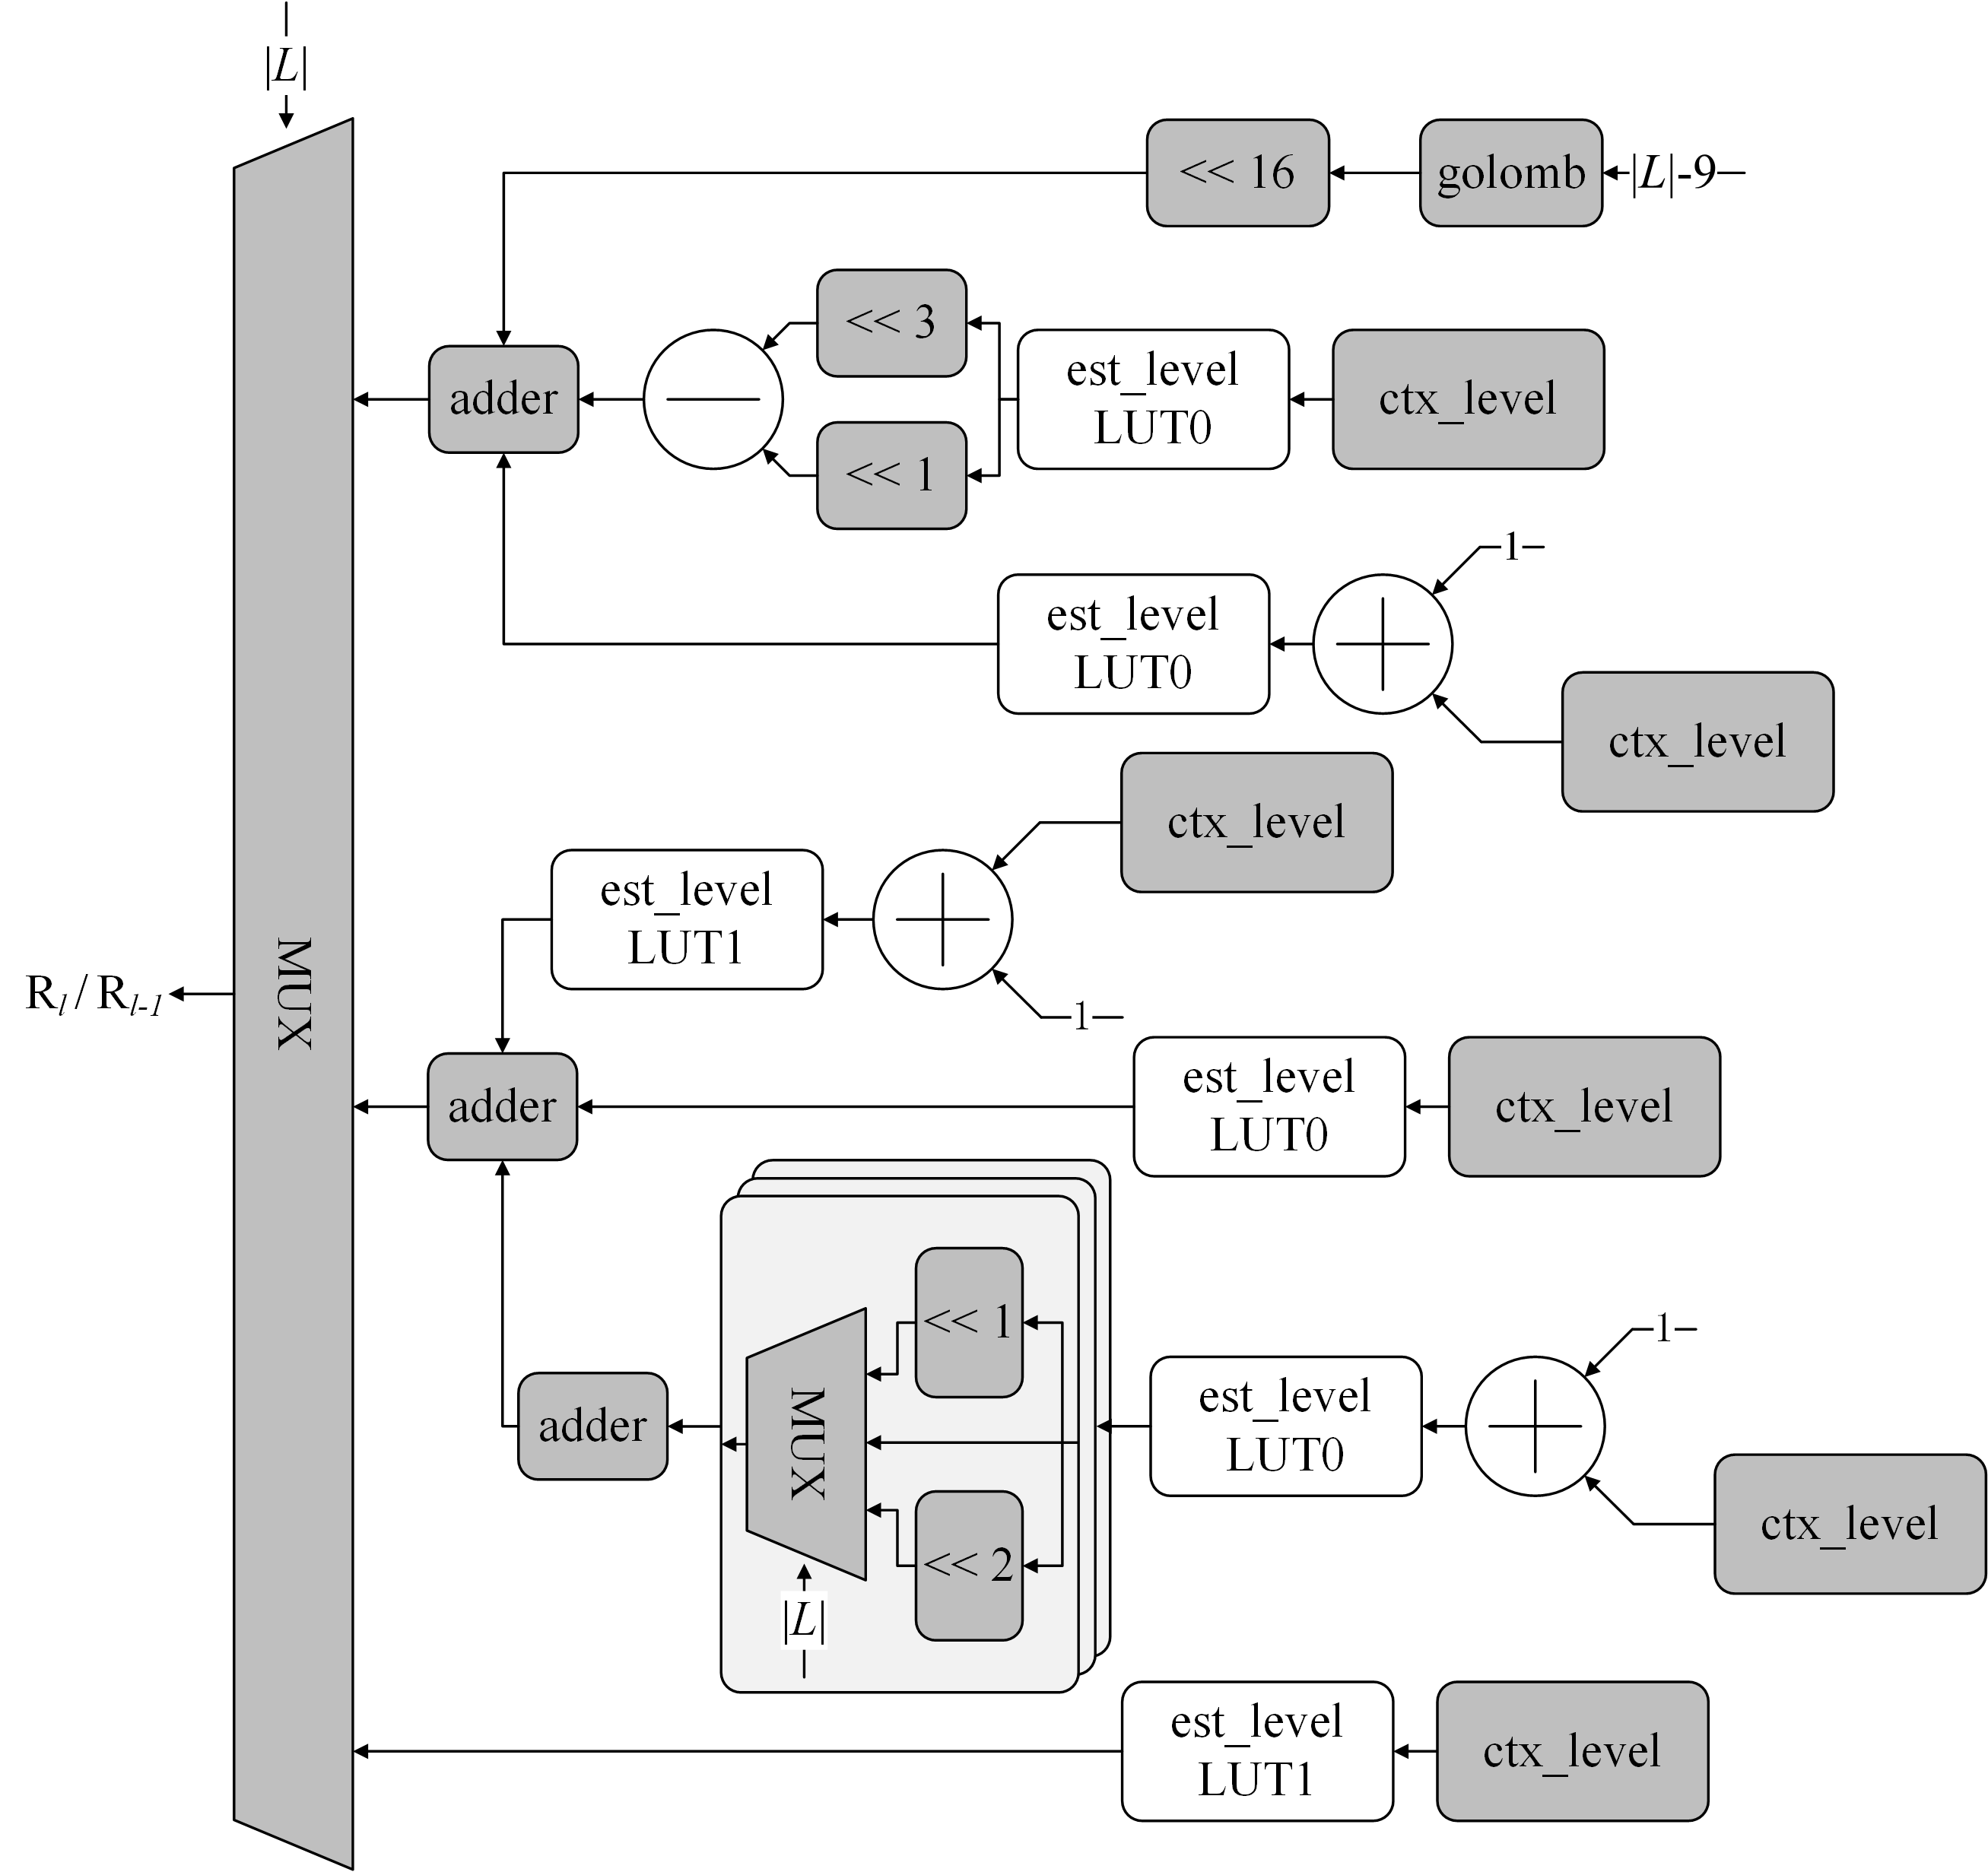
\includegraphics[width=0.49\textwidth]{pic_pan/rate_calculation.png}} 
	% figure caption is below the figure
	\caption{Three datapaths of the rate calculation architecture for $R_{l}$ and $R_{l-1}$.}
	\label{rate cost} % Give a unique label
\end{figure}

\subsection{LSC position decision}

The proposed greedy strategy based parallelized LSC position decision as outlined in subsection \ref{subsecgreedy}, effectively addresses the context dependency inherent in the zig-zag scan order. Consequently, the hardware architecture for the LSC position decision can be designed to incorporate high parallelism.

The proposed hardware architecture of the LSC position decision is scheduled from stage $S5$ to $S9$ as shown in Fig.~\ref{timing diagram}. This architecture can be further divided into three key components, each serving a distinct purpose.

The first component is following the determination of the minimum RD-cost as the optimal choice. The calculation of $\Delta J_{j}$, $E_{non_lsc}$, and $E_{lsc}$, as listed in Eq.~\eqref{A_i,last}, is scheduled at stage $S5$, preparing for the subsequent calculation of the optimal LSC position.

The second component is dedicated to making on-the-fly sub-optimal scanline LSC position decisions, where its used to calculate the optimal LSC position for the previous $W$ scanlines. This calculation is scheduled at the pipeline stage $S6$. 
Considering that the input to stage $S6$ is in a column-by-column manner, and each scanline in a single TU is in the up-right or down-left order. Thus, a shift hardware architecture is incorporated to align the temporal calculate results of each scanline, which corresponds to the for loop from line 28 to 30 in Algorithm \ref{the proposed LNPD algorithm}. 
Besides, the on-the-fly algorithm as described in subsection \ref{subsecgreedy} results in a sub-optimal position of an entire scanline being obtained in each cycle. Subsequently, a comparison is carried out between the obtained results and the previous scanlines, enabling the determination of the optimal position and its subsequent registration.

The remaining component focuses on calculating the optimal LSC decision for the remaining $H-1$ scanlines. This process is distributed across pipeline stages $S7$ to $S9$, facilitating the determination of the final optimal LSC positions.
Upon the final column of a given TU reaching the stage $S7$, all sub-optimal positions for each scanline are obtained. At this point, the computation process for determining the optimal LSC decision of the remaining $H-1$ scanlines commences.
Considering that the maximum height of the TU is 32, the process of comparing sub-optimal positions using a one-by-one sequence requires a total of 32 cycles. To minimize latency and enhance efficiency, the comparison of sub-optimal positions is executed in parallel, resulting in a reduction to just three cycles.
Take the TU with block size of 8$\times$8 for example. Once the last column of the TU enters stage S7, the two sub-optimal positions for each set of 4 scanlines are determined. These sub-optimal positions are then passed on to stage S8, where the final optimal position is obtained. Besides, the delay operation is adopted in $S9$ to align the output. Hence, the optimal LSC position is pipelined and outputted after a total of 40 ($6 + W_{max} - 1 + 3$) cycles.

\begin{figure*}[htbp]
	\centering
	\subfloat[]{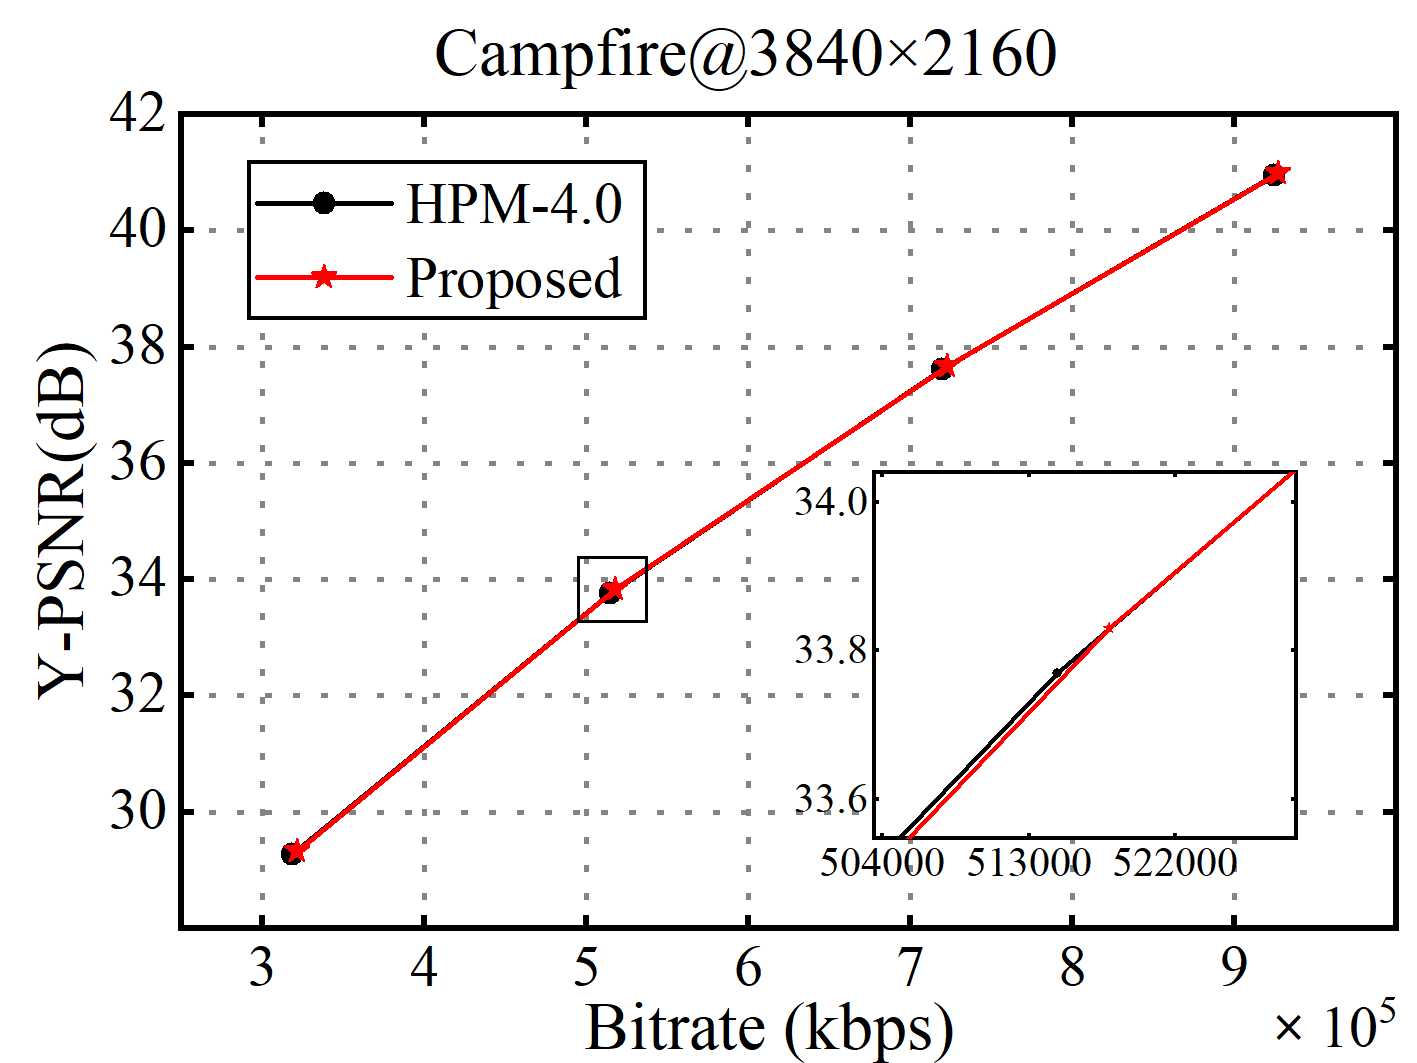
\includegraphics[width=.95\columnwidth]{figure/Campfire1.png}} \hspace{3pt}
	\subfloat[]{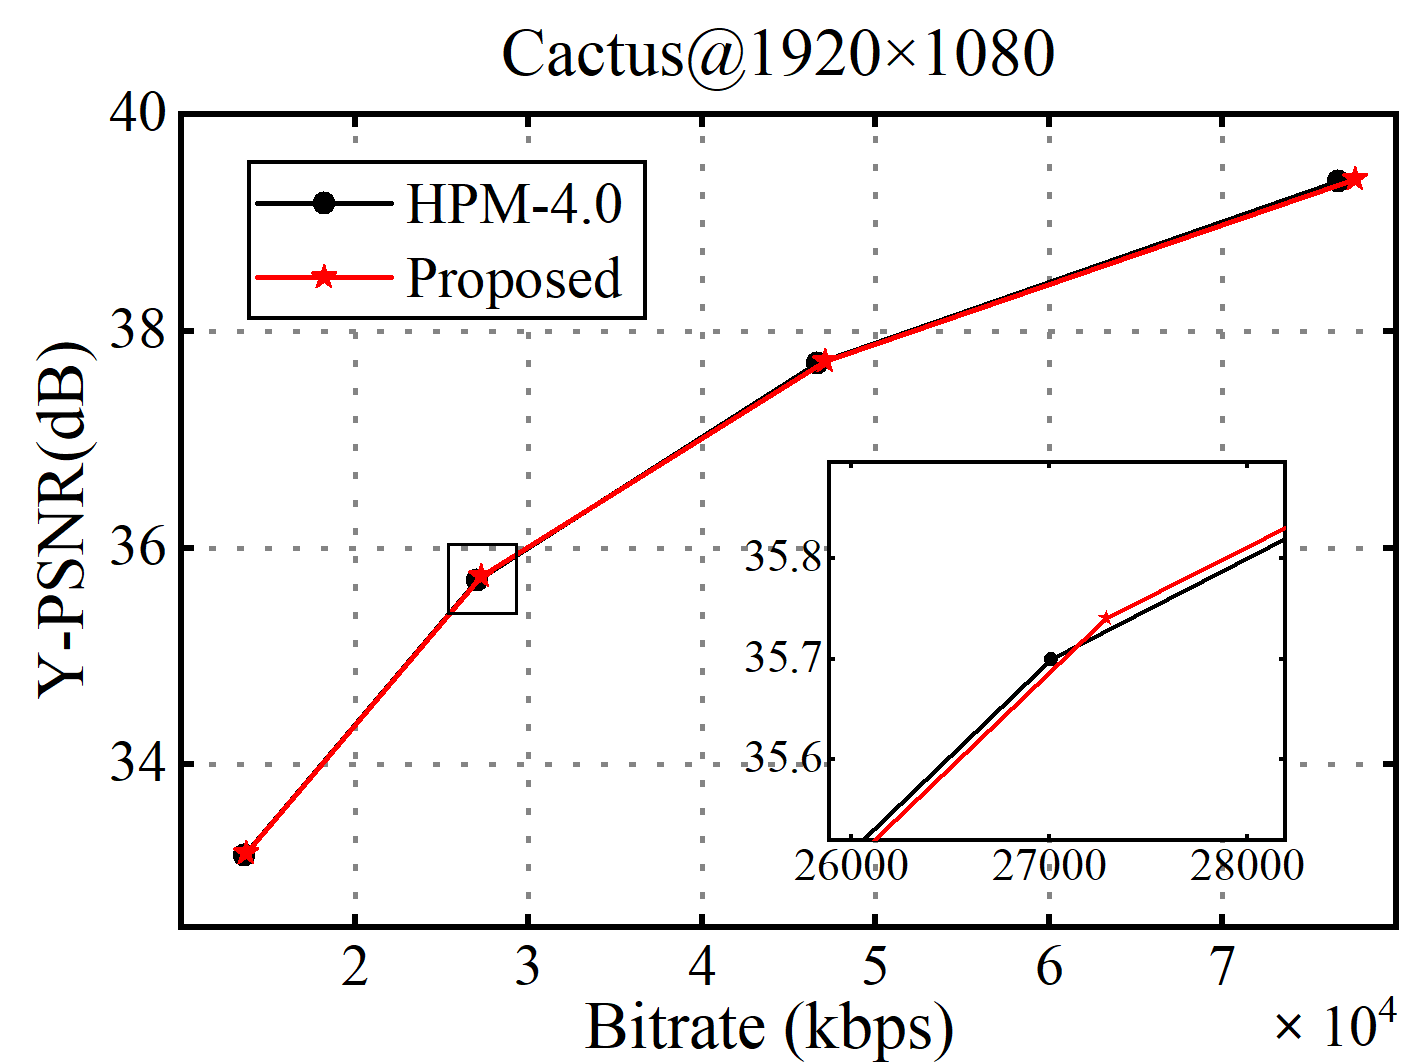
\includegraphics[width=.95\columnwidth]{figure/Cactus1.png}} \\
	\subfloat[]{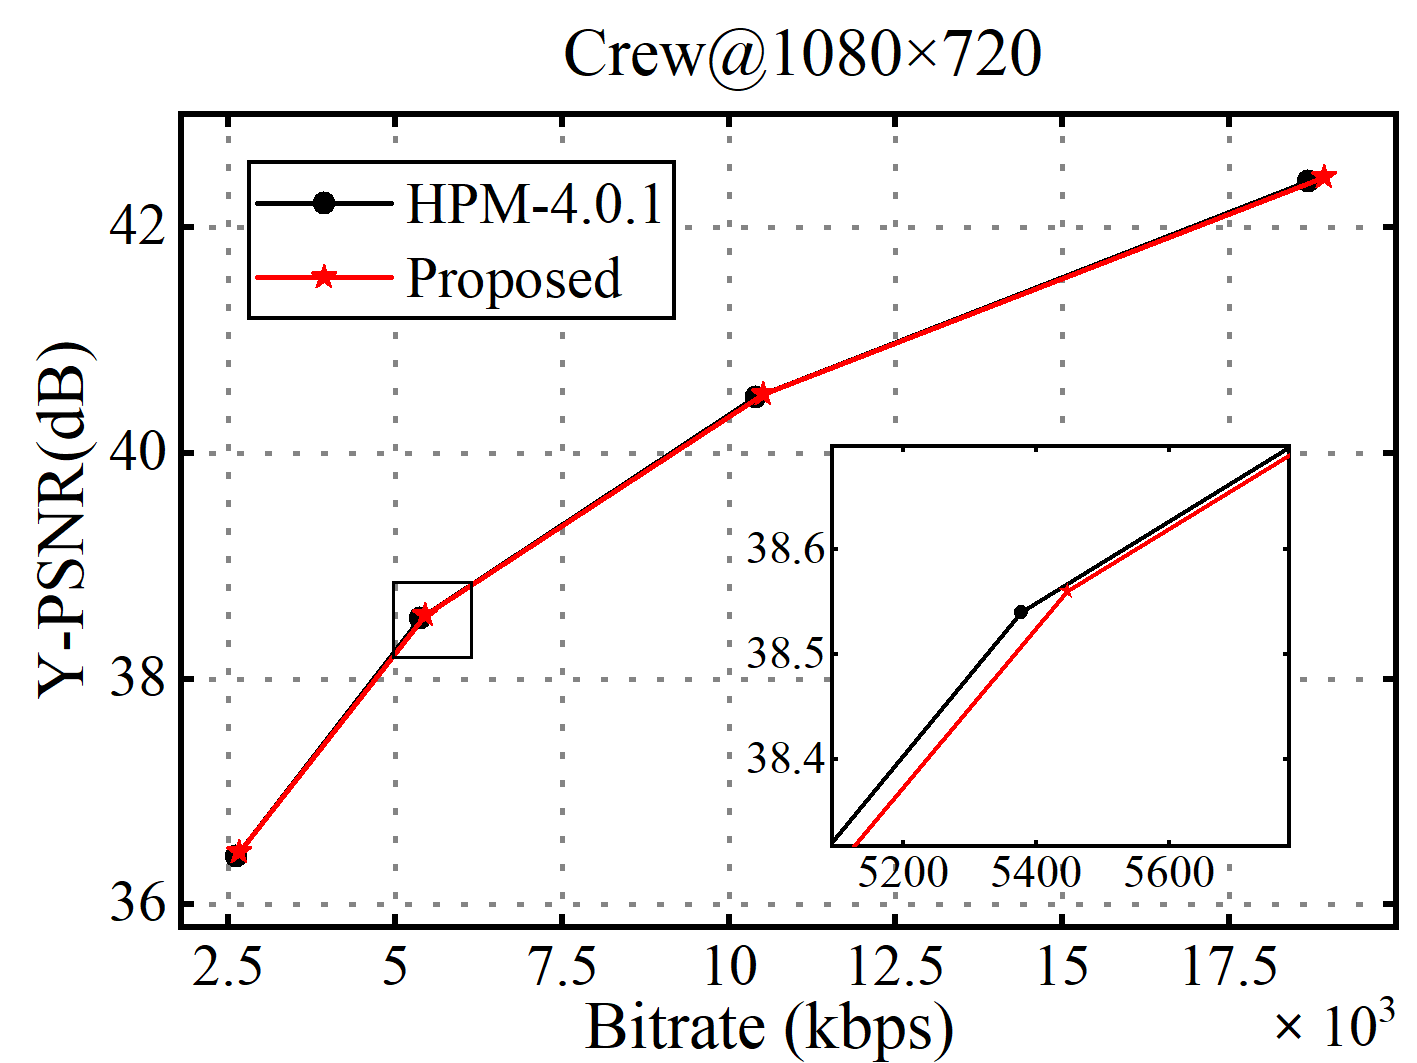
\includegraphics[width=.95\columnwidth]{figure/Crew1.png}} \hspace{3pt}
	\subfloat[]{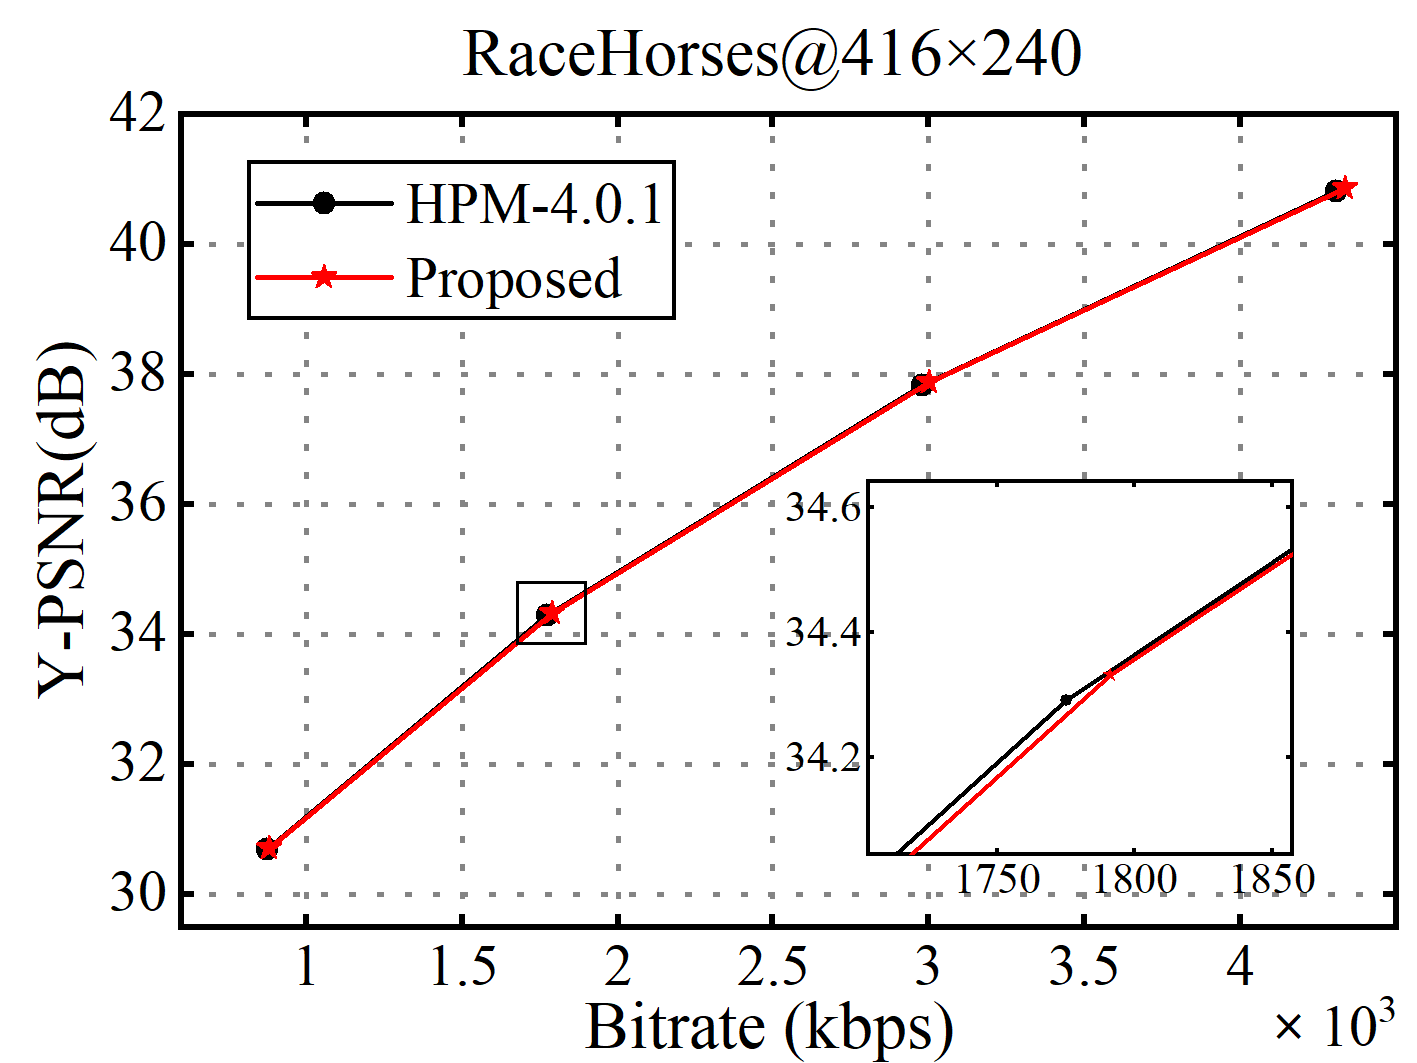
\includegraphics[width=.95\columnwidth]{figure/RaceHorses1.png}}
	\caption{RD curves for sequences Campfire, Cactus, Crew and RaceHorses with various resolution under AI configuration.}
    \label{RD curves}
\end{figure*}

\section{Experimental Results}
\label{sec:5}
In this section, software and hardware-related results are carried out and analyzed. Firstly, we describe the experimental environment setting. Then, we present and analyze the software-related results such as coding performance and computational complexity. Finally, we provide the hardware-related results including area, throughput, and power. 

\subsection{Experimental Settings} 
To validate the accuracy and efficiency of the proposed scheme, we implement the parallelized RDOQ algorithm in the AVS3 reference software HPM-4.0.1. The coding performance of the proposed algorithm is evaluated under AI, RA, and LDB configurations based on the AVS3 common test conditions (CTC) [xx]. We test 16 sequences in four categories, namely 240p (416×240), 720p (1280×720), HD (1920×1080), and UHD (4320×2160). The quantization parameters are set to 27, 32, 38, and 45. The coding performance is measured by BD-Rate and negative values represent performance gains \emph{TODO: cite}. The computational complexity of the proposed SIMD-based optimized parallelized RDOQ algorithm was measured by the actual encoding time. The test platform is Intel(R) Core(TM) i9-9900K CPU @ 3.60GHz. The time-saving $TS_{Q}$ of the RDOQ process and the time-saving $TS_{Esc}$ of the entire encoding process were obtained as follows, 
\begin{equation}
	\label{TSQ}
    TS_{Q} = \frac{T_{OriginQ}-T_{SIMDQ}}{T_{OriginQ}} \times 100\%,
\end{equation}

\begin{equation}
	\label{TSEnc}
	TS_{Enc} = \frac{T_{Origin}-T_{SIMD}}{T_{Origin}} \times 100\%,
\end{equation}
where $T_{OriginQ}$ and $T_{SIMDQ}$ represent the RDOQ time for the original and proposed SIMD-based parallelized schemes, respectively. Similarly, $T_{Origin}$ and $T_{SIMD}$ represent the total coding time for the original and proposed parallelized algorithm, respectively. 

\subsection{RD Performance and Computational Complexity Evaluation}
The overall experimental results that compared our parallelized RDOQ with vanilla HPM are presented in Table \ref{tab:BD-Rate}. Both the RD performance and time-saving results are evaluated under the AI, RA, and LDB configurations for each individual sequence in Table \ref{tab:BD-Rate}. It can be observed that the BD-Rate of the proposed parallelized RDOQ algorithm increases by 0.23\% in the AI configuration, 0.24\% in the RA configuration, and 0.26\% in the LDB configuration, respectively. The coding performance loss is insignificant, and the BD-Rate increment is relatively consistent across each sequence. Moreover, we show some R-D curves of several sequences in Fig. \ref{RD curves}. One sequence is selected from each video resolution, making total four sequences. These curves show that the BD-Rate of the proposed algorithm is very close to the original RDOQ in HPM-4.0.1, and the performance loss for these different resolution sequences fluctuates very small. 

In addition, we also give the time-saving results for proposed parallelized RDOQ algorithm based on SIMD in Table \ref{tab:BD-Rate}. It can be observed that the RDOQ process time is reduced by 31.42\%, 28.6\%, and 28.58\% under AI, RA, and LDB configurations on average, respectively. And, it can save 8.80\%, 6.84\%, and 6.96\% under AI, RA, and LDB configurations on average for the total encoding time. To evaluate the effect of QP on time-saving, we conduct tests for the $TS_{Q}$ results using four different resolution test sequences for comparison. As shown in Fig. \ref{Time curves}, as the QP value becomes larger, the more time is saved in the RDOQ process based on SIMD. This is because a higher QP value corresponds to a higher probability that the quantization coefficient will become zero, resulting in a higher chance that all the four parallelized coefficients in Fig. \ref{selection} become zero in the TU. When we accelerate the SIMD-based OCL decision process, we can skip the decision process if all four coefficients to be executed are zero. 

As analyzed above, the proposed scheme effectively reduces coding complexity while incurring insignificant RD performance loss compared to the original RDOQ. Furthermore, computation complexity has been significantly reduced. These results demonstrate that our proposed parallelized RDOQ method can achieve a well trade-off between coding performance and computational complexity. 

\subsection{Ablation Study}
In order to evaluate the effectiveness of the proposed method, we conduct ablation experiments in this subsection. In terms of the ablation study on coding performance, it is shown that the performance changes of the simplified run-level context, the improved RD cost form based on Eq.~\eqref{pRDcost}, and the greedy strategy-based LSC position decision are presented in Table \ref{Ablation:BD-Rate}. It is shown that the simplified run-level context gives a 0.23\%, 0.26\%, and 0.30\% BD-Rate increase under the AI, RA, and LDB configurations, respectively. The improved RD cost form shows a 0.00\% (0.23\%-0.23\%), -0.02\%(0.24-0.26), and -0.04\%(0.26\%-0.30\%) BD-Rate increase under the AI, RA, and LDB configurations, respectively. There is no BD-rate loss for the greedy strategy-based LSC position step. Therefore, the results indicate that the performance loss is primarily attributed to the simplified run-level context. And the improved RD cost form has a minimal effect, with some sequences even showing slight improvements. This is because the simplified run-level context remains the dependency for only the up-right scan lines, which impacts the rate calculation. Whereas, the improved RD cost form is affected only by a decimal precision error in the calculation of $D/\lambda$. The greed strategy-based LSC location decision has no coding efficiency impact because the dependency in the TU is moved to scanline level in the OCL decsion step. The optimized greed strategy-based LSC decision will not impact the final result from this point of view. 

In terms of ablation study on time-saving, the results on the three stages of SIMD optimization are tabulated in Table \ref{Ablation:Time}. The results show that the pre-quantization step using SIMD can achieve 21.53\%, 20.35\%, and 19.92\% time savings under the AI, RA, and LDB configurations, respectively. For the OCL decision step, an 8.94\% (30.47\% - 21.53\%), 7.01\% (27.36\% - 20.35\%) and 7.14\% (27.06\% - 19.92\%) time savings can be obtained, respectively. For the LSC location decision step, a 0.88\% (31.35\% - 30.47\%), 1.27\% (28.63\% - 27.36\%) and 1.5\% (28.56\% - 27.06\%) time saving is obtained, respectively. The results indicate that the pre-quantization step has the most significant time savings primarily due to its independent calculation process, which is more amenable to SIMD optimization. The reason for the poor optimization process of the LSC process is that the data in the look-up table needs to be exchanged between register and memory when calculating the rate. And for the LSC location decision step with the least time-saving, the reason for this derives from two factors. One is an improved parallel algorithm which has a time increase compared with the previous algorithm, due to the addition of a decision method for different scanlines and the calculation of multiple temporary variables, as shown in Algorithm \ref{the proposed LNPD algorithm}. The other is that when we optimize $if$ and $else\ if$ statements in Algorithm \ref{the proposed LNPD algorithm} based on SIMD, it needs the help of mask operation to achieve this function. The mask operation leads to a reduction in efficiency. 

\subsection{Performance Comparison with Other Methods} 
To validate the efficiency of our proposed scheme, a comparison between our method and five other existing methods are shown in in Table \ref{Compare:BD-Rate}. It is worth noting that these methods have been implemented on two different reference software platforms, namely HM (HEVC) and HPM (AVS3). For the work proposed on HM, we use the results from the original work for comparison directly. Since the parallel algorithm proposed in this paper is implemented on HPM-4.0.1, we re-implement the HPM platform-based algorithms and get the results for comparison. 

As shown in Table \ref{Compare:BD-Rate}, work \cite{lee2015fastquantizationmethod} and work \cite{xu2020simplifiedLevelEstimation} both speed up for the software platform, and they can achieve a time saving ranges from 12.9\% to 15.8\% with a negligible BD-Rate loss. Compared with \cite{lee2015fastquantizationmethod} and \cite{xu2020simplifiedLevelEstimation}, our parallelized algorithm can achieve more time saving with closely matched coding efficiency and focuses on the fully pipelined hardware implementation. Work \cite{igarashi2018parallelGPU} proposed a parallelized RDOQ algorithm for HEVC encoder. It achieves 4K@60fps real-time encoding on GPU with a significant 2.51\% BD-Rate loss. However, our proposed parallelized RDOQ algorithm achieves 4K@30FPS real-time encoding on FPGAs with only 0.24\% BD-Rate loss, which is a good trade-off between coding efficiency and hardware implementation. Work \cite{xu2022hardwarefriendlyforrdoq} introduces all-zero block skipping and an optimized rate estimation algorithm. It is shown that it obtains 27.6\% and 30.6\% time savings in the RA and LD configurations, respectively, but the BD-Rate loss is 0.86\% and 0.64\%. Our coding efficiency loss is smaller than work \cite{xu2022hardwarefriendlyforrdoq}. In addition, we add our previous work \cite{zhao2023scanline} into comparison as well, and it can be seen that the improved parallelized algorithm in this paper has better coding performance than in \cite{zhao2023scanline}. 

% As you can see from the Table \ref{Compare:BD-Rate}, work \cite{lee2015fastquantizationmethod} and work \cite{xu2020simplifiedLevelEstimation} both speed up in software by simplifying the RDOQ process, and they can achieve a time saving of 12.9\%-15.8\% with a negligible BD-Rate loss under AI, RA and LD configurations. Compared with \cite{lee2015fastquantizationmethod} and \cite{xu2020simplifiedLevelEstimation}, our parallel algorithm can achieve more time reduction with a close coding efficiency and mainly focus on the fully pipelined hardware implementation. Work \cite{igarashi2018parallelGPU} proposed a parallel RDOQ algorithm for HEVC encoder. It achieves 4K/60FPS real-time encoding on GPU with a high 2.51\% BD-Rate loss. Compared with \cite{igarashi2018parallelGPU}, our proposed parallel RDOQ algorithm achieves 4K/30FPS real-time encoding on FPGAs with only 0.24\% BD-Rate loss on average under RA configuration, which is a good trade-off between encoding performance and hardware implementation. Work \cite{xu2022hardwarefriendlyforrdoq} introduces all-zero block skipping and an optimized rate estimation algorithm. It can be seen that it obtains 27.6\% and 30.6\% time savings in the RA and LD configurations, respectively, but the BD-Rate loss is 0.86\% and 0.64\%. Compared to \cite{xu2022hardwarefriendlyforrdoq}, the BD-Rate loss of our proposed parallel scheme is only 0.24\% and 0.26\% with similar time savings in RA and LD configurations, respectively. In addition, we add our previous work \cite{zhao2023scanline} into comparison as well, and it can be seen that the improved parallel algorithm in this paper has better coding performance by comparing the BD-Rate in RA and LD configurations provided in \cite{zhao2023scanline}.

\subsection{Hardware Implementation Result}
The proposed hardware architecture has been implemented in Verilog and synthesized in FPGAs.

\begin{figure}[htbp]
	\centering
	\subfloat[]{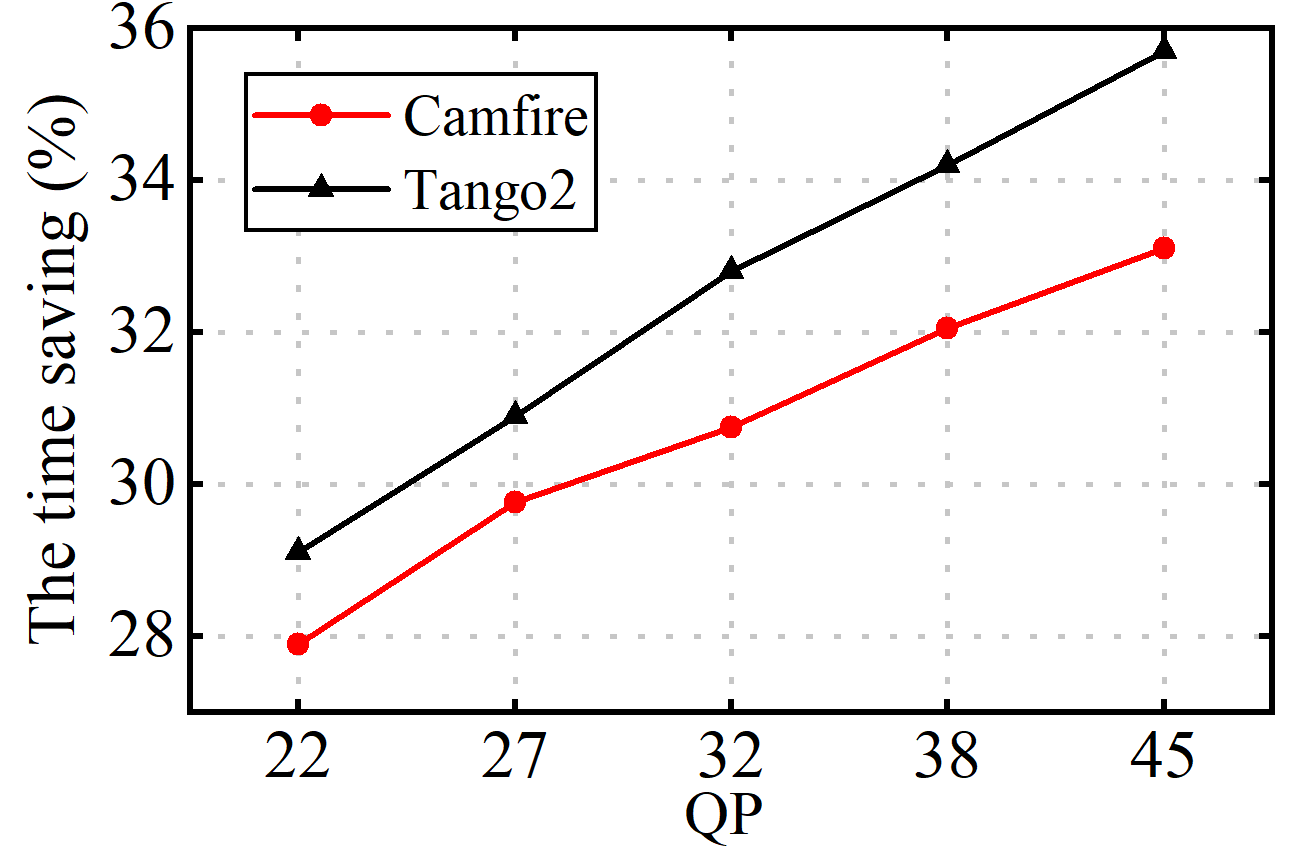
\includegraphics[width=.48\columnwidth]{figure/UHD.png}} \hspace{2pt}
	\subfloat[]{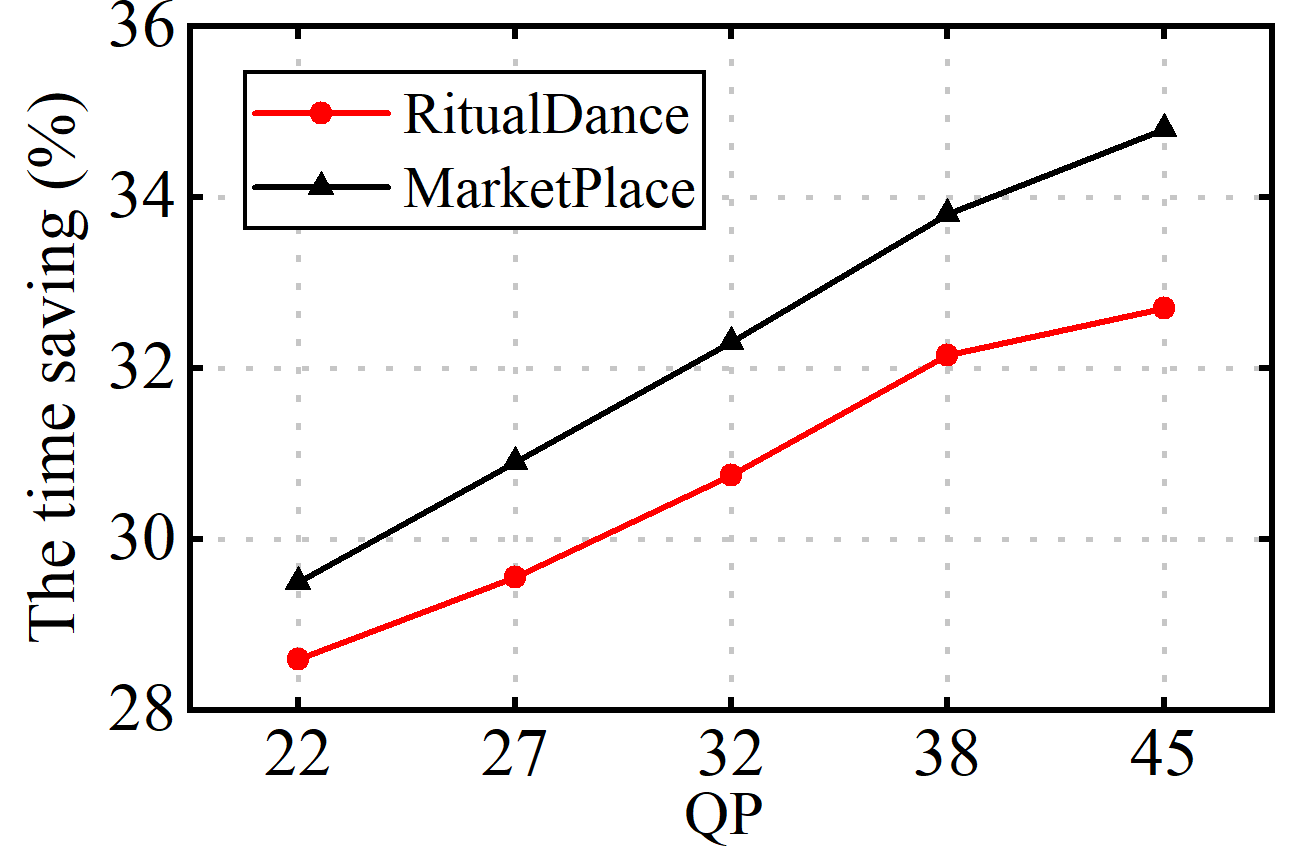
\includegraphics[width=.48\columnwidth]{figure/HD.png}} \vspace{-5pt} \\
	\subfloat[]{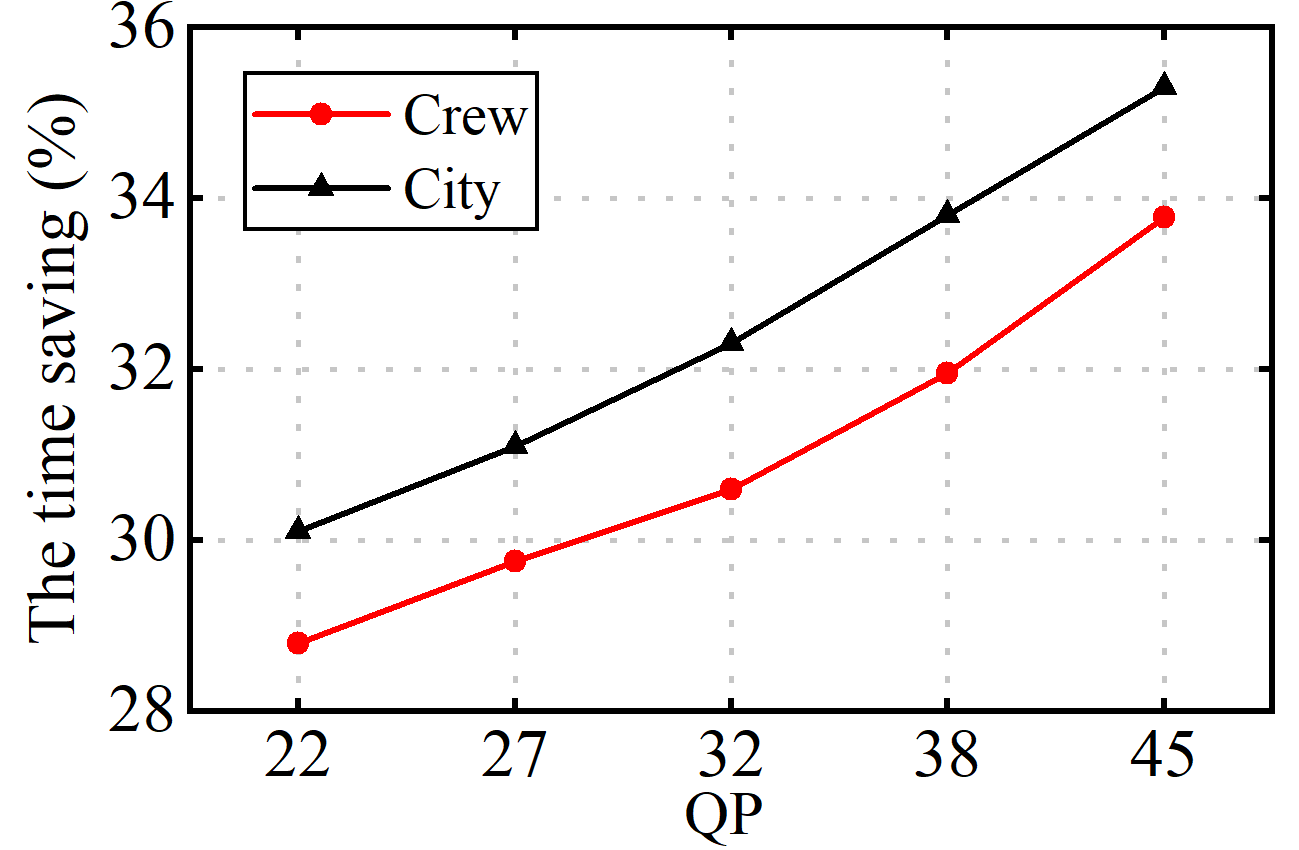
\includegraphics[width=.48\columnwidth]{figure/P720.png}} \hspace{2pt}
	\subfloat[]{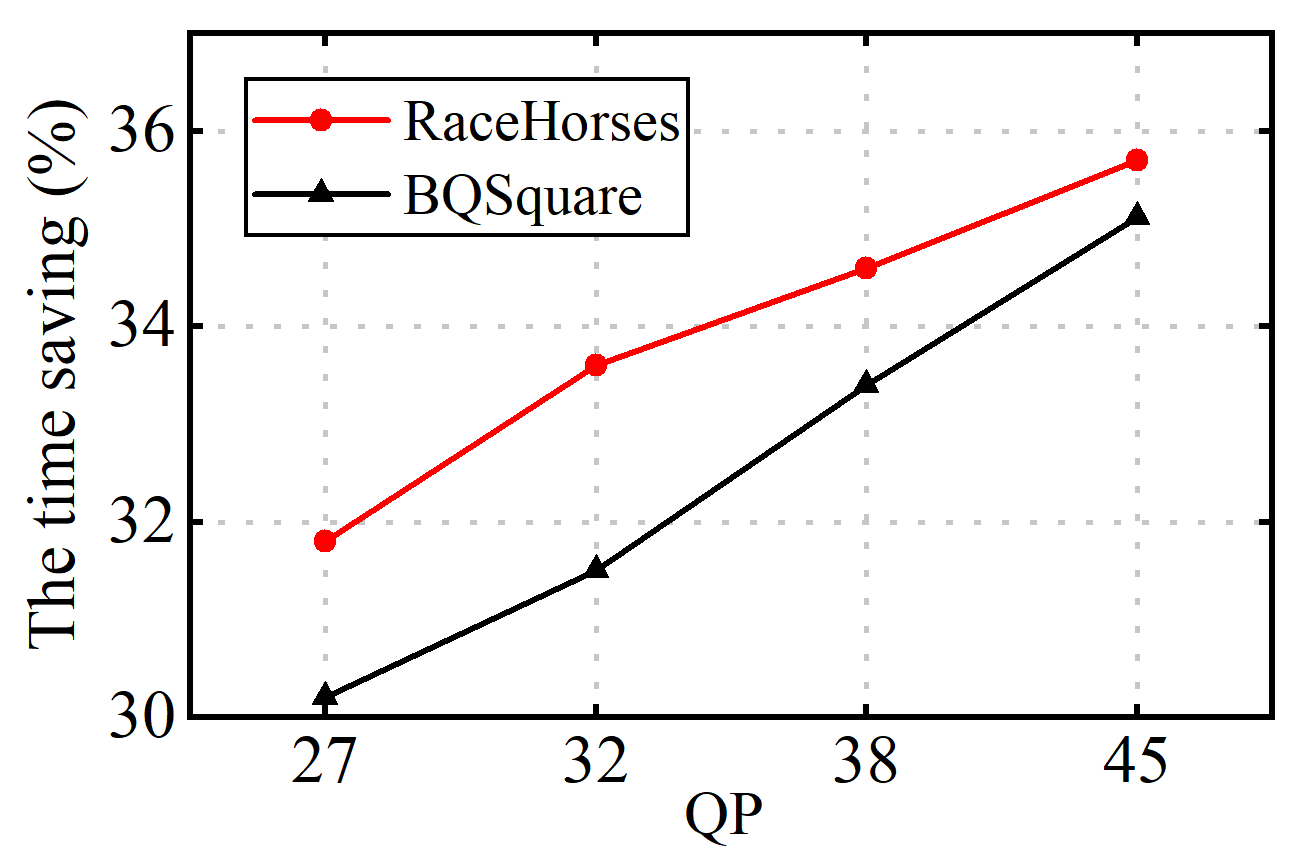
\includegraphics[width=.48\columnwidth]{figure/P240.png}}
	\caption{The time-saving results in the four sequence cases including UHD (a), HD (b), 720p (c) and 240p (d) under AI configuration.}
	\label{Time curves}
\end{figure}

\begin{table*}[!h]
	%\usepackage{hhline}
	\caption{BD-Rate of parallelized RDOQ in HPM-4.0.1 under AI, RA and LD configurations.}
    \label{tab:BD-Rate}
	\centering
	\tabcolsep 8pt  % 
	\arrayrulewidth 0.75pt
	\begin{tabular}{c | c | c   c   c | c   c   c | c   c   c } 
		\midrule[0.75pt] \specialrule{0em}{0.35pt}{0.35pt} \midrule[0.75pt] % \toprule
		\multirow{2}{*}{Class} & \multirow{2}{*}{Sequences} & \multicolumn{3}{c|}{AI} & \multicolumn{3}{c|}{RA} & \multicolumn{3}{c}{LDB} \\ 
		\cmidrule[0.75pt]{3-11} 
		       &                & BD-Rate & $TS_{Q}$ & $TS_{Enc}$ & BD-Rate & $TS_{Q}$ & $TS_{Enc}$ & BD-Rate & $ TS_{Q}$ & $TS_{Enc}$  \\   
		\cmidrule[0.75pt]{1-11}  
		       & Tango2         & 0.18\% & 33.36\% &10.21\% & 0.28\% & 29.96\% & 7.35\% & 0.28\% & 30.12\% & 8.03\% \\ 
		       & Parkrunning3   & 0.08\% & 30.12\% & 8.10\% & 0.17\% & 27.04\% & 6.29\% & 0.17\% & 27.64\% & 6.67\% \\  
		   UHD & Campfire       & 0.12\% & 31.42\% & 8.49\% & 0.34\% & 28.71\% & 7.02\% & 0.36\% & 27.92\% & 6.82\% \\           
	           & DaylightRoad2  & 0.08\% & 30.89\% & 8.31\% & 0.20\% & 27.95\% & 6.75\% & 0.19\% & 29.05\% & 7.15\% \\   
	    \cmidrule[0.75pt]{2-11} 
	           & Average        & 0.12\% & 31.45\% & 8.78\% & 0.25\% & 28.42\% & 6.85\% & 0.25\% & 28.68\% & 7.17\% \\ 
	    \cmidrule[0.75pt]{1-11}  
	           & Cactus         & 0.34\% & 30.75\% & 8.22\% & 0.21\% & 28.03\% & 6.47\% & 0.29\% & 27.91\% & 6.63\% \\          
	           & BasketballDrive& 0.45\% & 30.13\% & 8.12\% & 0.23\% & 27.12\% & 6.51\% & 0.34\% & 27.38\% & 6.45\% \\  
	      HD   & MarketPlace    & 0.18\% & 33.01\% & 9.97\% & 0.44\% & 30.69\% & 7.73\% & 0.22\% & 30.05\% & 7.29\% \\                    
	           & RitualDance    & 0.12\% & 31.29\% & 8.34\% & 0.31\% & 29.01\% & 7.13\% & 0.11\% & 29.89\% & 7.15\% \\   
	    \cmidrule[0.75pt]{2-11} 
	           & Average        & 0.28\% & 31.30\% & 8.66\% & 0.30\% & 28.71\% & 6.96\% & 0.24\% & 28.81\% & 6.88\% \\ 
	    \cmidrule[0.75pt]{1-11}  
	           & City           & 0.36\% & 33.11\% &10.02\% & 0.44\% & 29.55\% & 7.25\% & 0.53\% & 30.10\% & 8.11\% \\          
	           & Crew           & 0.36\% & 31.52\% & 8.56\% &-0.19\% & 28.88\% & 6.50\% & 0.41\% & 28.17\% & 6.39\% \\  
	     720p  & vidyo1         & 0.14\% & 30.43\% & 8.19\% & 0.34\% & 28.14\% & 6.44\% & 0.20\% & 27.35\% & 6.32\% \\             
	           & vidyo3         & 0.25\% & 29.52\% & 7.98\% & 0.13\% & 27.36\% & 6.27\% &-0.04\% & 27.64\% & 6.46\% \\   
	    \cmidrule[0.75pt]{2-11} 
	           & Average        & 0.28\% & 31.15\% & 8.69\% & 0.18\% & 28.48\% & 6.61\% & 0.28\% & 28.32\% & 6.82\% \\ 
	    \cmidrule[0.75pt]{1-11}  
	           & BasketballPass & 0.26\% & 31.59\% & 8.65\% & 0.14\% & 28.04\% & 6.38\% & 0.53\% & 27.82\% & 6.53\% \\          
	           & BQSquare       & 0.13\% & 32.56\% & 9.51\% & 0.50\% & 29.93\% & 7.28\% & 0.04\% & 29.05\% & 7.02\% \\  
	     240p  & BlowingBubbles & 0.35\% & 29.15\% & 7.84\% & 0.22\% & 27.03\% & 6.10\% & 0.39\% & 27.14\% & 6.27\% \\             
	           & RaceHorses     & 0.28\% & 33.91\% &10.28\% & 0.10\% & 30.12\% & 8.01\% & 0.21\% & 30.06\% & 8.08\% \\   
	    \cmidrule[0.75pt]{2-11} 
	           & Average        & 0.23\% & 31.80\% & 9.07\% & 0.24\% & 28.78\% & 6.94\% & 0.29\% & 28.52\% & 6.98\% \\ 
	    \cmidrule[0.75pt]{1-11} 
	    Summary & \textbf{Overall} & \textbf{0.23\%} & \textbf{31.42\%} & \textbf{8.80\%} & \textbf{0.24\%} & \textbf{28.60\%} & \textbf{6.84\%} & \textbf{0.26\%} & \textbf{28.58\%} & \textbf{6.96\%} \\ 
		\midrule[0.75pt] \specialrule{0em}{0.35pt}{0.35pt} \midrule[0.75pt] % \bottomrule
	\end{tabular}
\end{table*}


\begin{table}[!ht]
	%\usepackage{hhline}
	\caption{BD-Rate result of ablation study.}
	\label{Ablation:BD-Rate}
	\centering
	\tabcolsep 10pt  % 
	\arrayrulewidth 0.75pt
	\begin{tabular}{c | c  c  c } 
		\midrule[0.75pt] \specialrule{0em}{0.35pt}{0.35pt} \midrule[0.75pt] % \toprule
		\multirow{2}{*}{Method combination} & \multicolumn{3}{c}{BD-Rate} \\ 
		\cmidrule[0.75pt]{2-4} 
		& AI     & RA     & LDB \\   
		\cmidrule[0.75pt]{1-4}  
		Simplified run-level context                     & 0.23\% & 0.26\% & 0.30\% \\ 
		\cmidrule[0.75pt]{1-4}
		\makecell[c]{Simplified run-level context \\ + Optimized RD cost} & 0.23\% & 0.24\% & 0.26\%  \\
	    \cmidrule[0.75pt]{1-4}
		\makecell[c]{Simplified run-level context \\ + Optimized RD cost \\ + greedy strategy-based LSC \\ position decision} & 0.23\% & 0.24\% & 0.26\%  \\             
		\midrule[0.75pt] \specialrule{0em}{0.35pt}{0.35pt} \midrule[0.75pt] % \bottomrule
	\end{tabular}
\end{table}

\begin{table}[!ht]
	%\usepackage{hhline}
	\caption{Time-saving result of ablation study.}
	\label{Ablation:Time}
	\centering
	\tabcolsep 7pt  % 
	\arrayrulewidth 0.75pt
	\begin{tabular}{c | c  c  c } 
		\midrule[0.75pt] \specialrule{0em}{0.35pt}{0.35pt} \midrule[0.75pt] % \toprule
		\multirow{2}{*}{SIMD-based method combination} & \multicolumn{3}{c}{$TS_{Q}$} \\ 
		\cmidrule[0.75pt]{2-4} 
		& AI     & RA     & LDB \\   
		\cmidrule[0.75pt]{1-4}  
		Pre-quantization                      & 21.53\% & 20.35\% & 19.92\% \\ 
		\cmidrule[0.75pt]{1-4}
		Pre-quantization  + OCL decision      & 30.47\% & 27.36\% & 27.06\%  \\      
		\cmidrule[0.75pt]{1-4}
		\makecell[c]{Pre-quantization + OCL decision \\ + LSC position decision} & 31.35\% & 28.63\% & 28.56\%  \\            
		\midrule[0.75pt] \specialrule{0em}{0.35pt}{0.35pt} \midrule[0.75pt] % \bottomrule
	\end{tabular}
\end{table}

\begin{table}[!ht]
	%\usepackage{hhline}
	\caption{Comparasion of hardware resource consumption.}
	\label{hardware resource consumption}
	\centering
	\tabcolsep 7pt  % 
	\arrayrulewidth 0.75pt
	\begin{tabular}{c | c  c } 
		\midrule[0.75pt] \specialrule{0em}{0.35pt}{0.35pt} \midrule[0.75pt] 
		Design 		& \cite{zhao2023scanline}     & Proposed    \\   
		\cmidrule[0.75pt]{1-3}  
		LUTs   		& 109759 	& 72017 	\\ 
		\cmidrule[0.75pt]{1-3}
		FFs   		& 29576 	& 23440 	\\      
		\cmidrule[0.75pt]{1-3}
		DSPs  		& 481 		& 224 		\\     
		\cmidrule[0.75pt]{1-3} 
		Parallelism	& 32		& 32		\\
		\cmidrule[0.75pt]{1-3}
		Cycles  	& 538 		& 40		\\     
		\cmidrule[0.75pt]{1-3}
		Frequency  	& 200MHz	& 116MHz	\\            
		\midrule[0.75pt] \specialrule{0em}{0.35pt}{0.35pt} \midrule[0.75pt] 
	\end{tabular}
\end{table}

\begin{table*}[!ht]
	%\usepackage{hhline}
	\caption{Comparison with other works.}
	\label{Compare:BD-Rate}
	\centering
	\tabcolsep 8pt  % 
	\arrayrulewidth 0.75pt
	\begin{tabular}{c | c | c | c  c | c  c | c  c } 
		\midrule[0.75pt] \specialrule{0em}{0.35pt}{0.35pt} \midrule[0.75pt] % \toprule
		\multirow{2}{*}{Existing work} & \multirow{2}{*}{Reference software} & \multirow{2}{*}{Optimized for} & \multicolumn{2}{c|}{AI} & \multicolumn{2}{c|}{RA} & \multicolumn{2}{c}{LDB} \\ 
		\cmidrule[0.75pt]{4-9} 
		&        &        & BD-Rate & $TS_{Q}$ & BD-Rate & $TS_{Q}$ & BD-Rate & $ TS_{Q}$\\   
		\cmidrule[0.75pt]{1-9}
		Work \cite{lee2015fastquantizationmethod}   & HM 11.0   & Software & 0.09\% & 14.4\% & 0.11\% & 15.8\% & 0.08\% & 14.9\% \\ 
		\cmidrule[0.75pt]{1-9}  
		Work \cite{xu2020simplifiedLevelEstimation} & HM 16.15  & Software & 0.00\% & 14.4\% & 0.04\% & 12.9\% & 0.12\% & 12.9\% \\ 
		\cmidrule[0.75pt]{1-9} 
		Work \cite{igarashi2018parallelGPU}         & HM 16.0   & Hardware & N/A    & N/A    & 2.51\% & N/A    & N/A    & N/A  \\ 
		\cmidrule[0.75pt]{1-9}
		Work \cite{xu2022hardwarefriendlyforrdoq}   & HPM-4.0.1 & Hardware & N/A    & N/A    & 0.86\% & 27.6\% & 0.64\% & 30.6\% \\     
		\cmidrule[0.75pt]{1-9}      
		Work \cite{zhao2023scanline}                & HPM-4.0.1 & Hardware & 0.82\% & N/A    & 0.46\% & N/A    &  0.36\%   & N/A \\   
		\cmidrule[0.75pt]{1-9}  
		Proposed                                    & HPM-4.0.1 & Hardware & 0.23\% & 31.4\% & 0.24\% & 28.6\% & 0.26\% & 28.58\%  \\          
		\midrule[0.75pt] \specialrule{0em}{0.35pt}{0.35pt} \midrule[0.75pt] % \bottomrule
	\end{tabular}
\end{table*}



\section{Conclusion and Future Work}
\label{sec:6}
In this paper, a parallelized RDOQ algorithm and its fully pipelined hardware architecture design is presented for AVS3 video coding standard. For the parallelized algorithm, the run-level context for the rate estimation is updated in the inner zig-zag scanline and an efficient RD cost form is adopted in the OCL decision step. In the LSC position decision step, a greedy strategy-based algorithm is proposed to achieve the LSC position decision compute in parallel. Moreover, the parallelized algorithm is accelerated based on SIMD. The experimental results show that the BD-rate of the parallelized algorithm is increased by 0.23\%, 0.24\%, and 0.26\% under the AI, RA, and LDB configurations, respectively. The computational time is reduced by 31.42\%, 28.60\%, and 28.58\% compared to the vanilla HPM-4.0.1, respectively. 
For the hardware architecture, we design a ... is capable of performing real-time video coding up to 30 fps of 4K using ... Furthermore, due to the strong similarity for scanning in TU among the AVS3, HEVC and VVC encoders. 
In our future study, we will extend the proposed parallelized algorithm to RDOQ in HEVC and explore novel methods to speed-up the dependent quantization computation in VVC. 

% \section*{Acknowledgments}
% This should be a simple paragraph before the References to thank those individuals and institutions who have supported your work on this article. 

%{\appendix[Proof of the Zonklar Equations]
%Use $\backslash${\tt{appendix}} if you have a single appendix:
%Do not use $\backslash${\tt{section}} anymore after $\backslash${\tt{appendix}}, only $\backslash${\tt{section*}}.
%If you have multiple appendixes use $\backslash${\tt{appendices}} then use $\backslash${\tt{section}} to start each appendix.
%You must declare a $\backslash${\tt{section}} before using any $\backslash${\tt{subsection}} or using $\backslash${\tt{label}} ($\backslash${\tt{appendices}} by itself
% starts a section numbered zero.)}

%{\appendices
%\section*{Proof of the First Zonklar Equation}
%Appendix one text goes here.
% You can choose not to have a title for an appendix if you want by leaving the argument blank
%\section*{Proof of the Second Zonklar Equation}
%Appendix two text goes here.}

\bibliographystyle{IEEEtran}
\bibliography{References}
\end{document}